%%%% utfpr-thesis.tex, 2025/08/03
%%%% Copyright (C) 2021-2025 Luiz E. M. Lima (luizeduardomlima@gmail.com)
%%
%% This work may be distributed and/or modified under the conditions of the
%% LaTeX Project Public License, either version 1.3 of this license or (at your
%% option) any later version.
%% The latest version of this license is in
%%   https://www.latex-project.org/lppl.txt
%% and version 1.3 or later is part of all distributions of LaTeX version
%% 2005/12/01 or later.
%%
%% This work has the LPPL maintenance status `maintained'.
%%
%% The Current Maintainer of this work is Luiz E. M. Lima.
%%
%% This work consists of all files listed in readme.html.
%%
%% A brief description of this work is in readme.txt.

%% Conformidade com PDF/A (LaTeX release 2022-06-01 or later)
% \DocumentMetadata{pdfstandard = A-3b, pdfversion = 1.7, lang = pt-BR}

%% Detecção e aviso sobre comandos obsoletos
% \RequirePackage[l2tabu, orthodox]{nag}

%% Classe de documento
\documentclass[%% Opções (^ = padrão; > = para pacotes; ¹ = somente twoside):
  a4paper,%% Tamanho de papel: a4paper, letterpaper (^), etc.
  12pt,%% Tamanho de fonte: 9pt, 10pt (^), 11pt, 12pt, 14pt, etc.
  oneside,%% Impressão de folhas: oneside ou twoside (^)
%   openany,%% Impressão de capítulos (¹): openany ou openright (^)
%   fleqn,%% Alinhamento de equações à esquerda (centralizado por padrão)
%   draft,%% Aparência de documento (>): draft ou final (^)
  english,%% Idioma secundário (penúltimo) (>)
  brazilian,%% Idioma primário (último) (>)
]{memoir}

%% Pacotes utilizados
\usepackage[%% Opções (^ = padrão; ¹ = somente twoside; ² = somente openany):
%   Version   = Abstract,%% Versão de documento: Final (^), Defense ou Abstract
%   Font      = Times,%% Fonte principal: Arial (^), Calibri, Times ou LaTeX(*)
%   LinkColor = ,%% Cor (HTML) hyperlink (azul escuro ^): nenhuma (cor texto)
%   CoverBG   = On,%% Planos de fundo (Capa e Contracapa): On ou Off (^)
%   CoverData = All,%% Dados de identificação (Capa): All ou Main (^)
%   PageNum   = All,%% Numeração de páginas (partes): All, Main (^) ou None
%   TwoSide   = All,%% Frente e verso (partes) (¹): All, Main (^) ou None
%   OpenPage  = Odd,%% Paginação de elementos (²): Odd ou Any (^)
%   ApxAnxTtl = Lower,%% Título (case) de apêndices e anexos: Lower ou Upper (^)
%   Caption   = Left,%% Alinhamento de legendas: Center (^) ou Left
%   Source    = Left,%% Alinhamento de fontes (autoria): Center (^) ou Left
%   ABNTCit   = NSB,%% Citação ABNT: AAY (Nome, Ano) (^), NRB (1) ou NSB [1]
%   DOIIcon   = On,%% Ícone de DOI em referências: On ou Off (^)
%   URLIcon   = On,%% Ícone de URL em referências: On ou Off (^)
]{utfpr-thesis}

%% Informações do documento (descomentar para alterar; * = opcional)
%%%% Título: [Original: brazilian ou english]; {Português}; {English}
% \Title{%
%   Título de trabalho acadêmico%
% }{%
%   Title of academic work%
% }
%%%% Subtítulo (*): {Português}; {English}
% \SubTitle{%
%   subtítulo de trabalho acadêmico%
% }{%
%   subtitle of academic work%
% }
%%%% Aluno(s) (de 1 a 5): {Número}; {Dados}
% \Student{1}{%
%   Gender   = {Male},%% Ou {Female}
%   Forename = {Prenome{(s)}},%% Exceto último e sufixo, e.g., {José Santos da}
%   Surname  = {Sobrenome-A1},%% Último e sufixo, e.g., {Silva Júnior}
%   Email    = {student1@domain},%% (*)
%   Lattes   = {0000000000010001},%% (*)
%   ORCID    = {0000-0000-0001-0001},%% (*) (CHKTEX 8)
% }
%%%% Grau acadêmico (opção; ¹ = automático para cada opção): [Número]
% \AcademicDegreeOption[1]%% Doutorado
% \AcademicDegreeOption[2]%% Mestrado
% \AcademicDegreeOption[3]%% Especialização
% \AcademicDegreeOption[4]%% Bacharelado
% \AcademicDegreeOption[5]%% Licenciatura
% \AcademicDegreeOption[6]%% Tecnologia
%%%%%% Grau acadêmico (¹): {Português}; {English}
% \AcademicDegree{Doutorado}{Doctorate}
%%%%%% Título acadêmico (¹): {Português}; {English}
% \AcademicTitle{Doutor\Gen{a}}{Doctor}
%%%%%% Tipo de documento (¹): {Português}; {English}
% \DocumentType{Tese}{Thesis}
%%%% Curso(s): {Português}; {English}
% \Course{Engenharia Mecânica}{Mechanical Engineering}
%%%% Departamento(s), coordenação(ões) ou programa: {Português}; {English}
% \Department{%
%   Programa de Pós-Graduação em Engenharia Mecânica%
% }{%
%   Mechanical Engineering Graduate Program%
% }
%%%% Campus: {Cidade}
% \Campus{Ponta Grossa}
%%%% Data(s) (atual por padrão): [Ano (depósito)]; {Ano (defesa)}; {Mês}; {Dia}
% \Dates{2025}{12}{31}

%% Processamento (makeindex) de entradas (itens) de listas, glossários e índices
%%%% Lista de Abreviaturas e Siglas: [Arquivo de Entradas]
% \MakeAcronyms[./Pre-Textual/Optionals/acronyms-entries]%% Sem subdivisões
% \MakeAcronyms*[./Pre-Textual/Optionals/acronyms-entries]%% Com subdivisões
%%%% Lista de Símbolos: [Arquivo de Entradas]
% \MakeSymbols[./Pre-Textual/Optionals/symbols-entries]%% Sem subdivisões
% \MakeSymbols*[./Pre-Textual/Optionals/symbols-entries]%% Com subdivisões
%%%% Glossário: [Arquivo de Entradas]
% \MakeGlossary[./Post-Textual/Optionals/glossary-entries]
%%%% Índice Remissivo
% \MakeIndex%

%% Controle de inclusão de arquivos via \include (comentar para desativar)
\includeonly{%
  ./Chapter-1/chapter-1,%% Capítulo 1 (CHKTEX 26)
  ./Chapter-2/chapter-2,%% Capítulo 2 (CHKTEX 26)
  ./Chapter-3/chapter-3,%% Capítulo 3 (CHKTEX 26)
  ./Chapter-4/chapter-4,%% Capítulo 4 (CHKTEX 26)
  ./Chapter-5/chapter-5,%% Capítulo 5 (CHKTEX 26)
  ./Chapter-Example/chapter-example,%% Capítulo de exemplo (CHKTEX 26)
  ./Post-Textual/appendix-a,%% Apêndice A (CHKTEX 26)
  ./Post-Textual/appendix-b,%% Apêndice B (CHKTEX 26)
  ./Post-Textual/annex-a,%% Anexo A (CHKTEX 26)
  ./Post-Textual/annex-b,%% Anexo B (CHKTEX 26)
}

%% Arquivo(s) de referências
\addbibresource{./Post-Textual/references-examples.bib}
\addbibresource{./Post-Textual/references.bib}

%% Início do documento
\begin{document}

%% Capa (automática)
%% Para inserir planos de fundo na Capa e em uma Contracapa:
%% a) selecionar a opção do pacote utfpr-thesis: CoverBG = On;
%% b) atribuir nas informações do documento argumentos válidos para:
%%    - grau acadêmico (\AcademicDegreeOption[Número]);
%%    - campus (\Campus{Cidade}).

%% Elementos pré-textuais (frontmatter)
%% Editar o {Arquivo} para alterar: Folha de Rosto, Errata, Folha de Aprovação,
%% Dedicatória, Agradecimentos, Epígrafe, Resumo e Abstract.
%%%% Elementos pré-textuais (opcionais)
%%
%% Lista de Ilustrações, Lista de Tabelas, Lista de Abreviaturas e Siglas, Lista
%% de Símbolos e Sumário.
%%
%% Tamanho de fonte
% \csletcs{listfontsize}{footnotesize}

%% Lista de Ilustrações (somente se houver muitas ilustrações)
\listoffigures%

%% Lista de Tabelas (somente se houver muitas tabelas)
\listoftables%

%% Lista de Abreviaturas e Siglas (inserir itens em ordem alfabética)
\begin{AcronymsList}%[Título Alternativo]%% Substitui o título padrão
\item[ABNT] Associação Brasileira de Normas Técnicas
\item[CTAN] \ENLang{Comprehensive \TeX\ Archive Network}
\item[NBR] Norma Brasileira
\item[PDF] Formato de Documento Portátil (\ENLang*{Portable Document Format})
\item[QR] Resposta Rápida (\ENLang*{Quick Response})
\item[TUG] \ENLang{\TeX\ Users Group}
\item[URL] Localizador Uniforme de Recursos (\ENLang*{Uniform Resource Locator})
\item[UTFPR] Universidade Tecnológica Federal do Paraná
\end{AcronymsList}

%% Lista de Símbolos (inserir itens em ordem de ocorrência)
\begin{SymbolsList}%[Título Alternativo]%% Substitui o título padrão
\item[u] Velocidade, \Unit{m/s}
\item[\beta] Amplitude de velocidade, \Unit{m/s}
\item[\pi] Constante circular (Pi), \Unit{rad}
\item[A] Área, \Unit{m^2}
\item[\mathrm{Re}] Número de Reynolds
\end{SymbolsList}

%% Sumário (somente se houver muitas seções)
\tableofcontents%

%% Para finalizar o documento nos elementos Resumo e Abstract, selecionar a
%% opção do pacote utfpr-thesis: Version = Abstract.
\EndDocumentVersionAbstract%% Fim do documento na versão Resumo

%% Lista de Algoritmos (elemento opcional)
% \PrintFloatsList{algorithm}

%% Lista (geral) de Ilustrações (elemento opcional)
% \PrintIllustrationsList{figure, flowchart, photograph, graph, tabframed}
%%%% Lista de Figuras (usar a partir de 3 itens e remover da lista geral)
% \PrintFloatsList{figure}
%%%% Lista de Fluxogramas (usar a partir de 3 itens e remover da lista geral)
% \PrintFloatsList{flowchart}
%%%% Lista de Fotografias (usar a partir de 3 itens e remover da lista geral)
% \PrintFloatsList{photograph}
%%%% Lista de Gráficos (usar a partir de 3 itens e remover da lista geral)
% \PrintFloatsList{graph}
%%%% Lista de Quadros (usar a partir de 3 itens e remover da lista geral)
% \PrintFloatsList{tabframed}

%% Lista de Tabelas (elemento opcional)
% \PrintFloatsList{table}

%% Lista de Abreviaturas e Siglas (elemento opcional)
%%%% Opção 1 (makeindex; conforme o [Arquivo de Entradas] em \MakeAcronyms)
% \PrintAcronymsList%
%%%% Opção 2 (manual; editar o {Arquivo} para alterar)
% %%%% LISTA DE ABREVIATURAS E SIGLAS (ELEMENTO OPCIONAL)
%%
%% Consiste na relação alfabética das abreviaturas e siglas utilizadas no texto,
%% seguidas das palavras ou expressões correspondentes grafadas por extenso.
%% Recomenda-se a elaboração de lista própria para cada tipo.
\begin{AcronymsList}%[Título Alternativo]%% Substitui o título padrão
\item[1D] Unidimensional
\item[ABNT] Associação Brasileira de Normas Técnicas
\item[Art.] Artigo
\item[BMP] Mapa de Bits (\ENLang*{Bitmap})
\item[Cap.] Capítulo
\item[CAPES] Coordenação de Aperfeiçoamento de Pessoal de Nível Superior
\item[CNPq] Conselho Nacional de Desenvolvimento Científico e Tecnológico
\item[CTAN] \ENLang{Comprehensive \TeX\ Archive Network}
\item[EPS] \ENLang{Encapsulated PostScript}
\item[GIF] Formato de Intercâmbio de Gráficos (\ENLang*{Graphics Interchange Format})
\item[GIMP] Programa de Manipulação de Imagem GNU (\ENLang*{GNU Image Manipulation Program})
\item[GNU] GNU Não é Unix (\ENLang*{GNU is Not Unix})
\item[JPEG] \ENLang{Joint Photographic Experts Group}
\item[NBR] Norma Brasileira
\item[PDF] Formato de Documento Portátil (\ENLang*{Portable Document Format})
\item[PNG] Gráficos Portáteis de Rede (\ENLang*{Portable Network Graphics})
\item[PS] \ENLang{PostScript}
\item[QR] Resposta Rápida (\ENLang*{Quick Response})
\item[Seç.] Seção
\item[TCC] Trabalho de Conclusão de Curso
\item[TUG] \ENLang{\TeX\ Users Group}
\item[UML] Linguagem de Modelagem Unificada (\ENLang*{Unified Modeling Language})
\item[URL] Localizador Uniforme de Recursos (\ENLang*{Uniform Resource Locator})
\item[UTF-8] Formato de Transformação Unicode de 8-bit (\ENLang*{8-bit Unicode Transformation Format})
\item[UTFPR] Universidade Tecnológica Federal do Paraná
\end{AcronymsList}


%% Lista de Símbolos (elemento opcional)
%%%% Opção 1 (makeindex; conforme o [Arquivo de Entradas] em \MakeSymbols)
% \PrintSymbolsList%% Unidade após descrição (separada por ,)
% \PrintSymbolsList*%% Unidade na margem direira (entre [])
%%%% Opção 2 (manual; editar o {Arquivo} para alterar)
% %%%% LISTA DE SÍMBOLOS (ELEMENTO OPCIONAL)
%%
%% Conjunto de sinais que substituem o nome de uma coisa ou de uma ação.
%% Elaborada conforme a ordem apresentada no texto, com o devido significado.
\begin{SymbolsList}%[Título Alternativo]%% Substitui o título padrão
\item[\nu] Viscosidade cinemática, \Unit{m^2/s}
\item[\mu] Viscosidade dinâmica, \Unit{kg/{(m{\cdot}s)}}
\item[\rho] Massa específica, \Unit{kg/m^3}
\item[A] Área, \Unit{m^2}
\item[\pi] Constante circular, \Unit{rad}
\item[D] Diâmetro, \Unit{m}
\item[R] Raio, \Unit{m}
\item[\overline{\MrkSym}] Média temporal
\item[\langle\MrkSym\rangle] Média na seção transversal
\item[\vec{\nabla}] Operador gradiente
\item[\MrkSym^-] Passo de tempo anterior
\item[\MrkSym^+] Passo de tempo posterior
\item[\MrkSym^0] Valor inicial
\item[\MrkSym_\mathrm{G}] Fase gasosa
\item[\MrkSym_\mathrm{L}] Fase líquida
\item[\MrkSym_\mathrm{S}] Fase sólida
\item[\theta] Inclinação, \Unit{\Degree}
\item[L] Comprimento, \Unit{m}
\item[\mathrm{Re}] Número de Reynolds
\item[V] Velocidade, \Unit{m/s}
\end{SymbolsList}


%% Sumário
\PrintSummary%% Com espaçamento entre partes e entre capítulos
% \PrintSummary*%% Sem espaçamento entre partes e entre capítulos

%% Formatação de elementos textuais (mainmatter; não comentar ou remover)
\Textual%

%% Parte 1 (elemento opcional; agrupamento de capítulos)
% \part{Introdução}%
% \label{part:intro}

%% Capítulo 1
%%%% CAPÍTULO 1: INTRODUÇÃO
%%
%% Deve apresentar uma visão global da pesquisa, incluindo: breve histórico,
%% importância e justificativa de escolha do tema, delimitações do assunto,
%% formulação de hipóteses, objetivos da pesquisa e estrutura do trabalho.

%% Locais (pastas) de ilustrações deste capítulo
\graphicspath{%
  {./Chapter-1/}%% Primário
%   {./Chapter-1/Illustrations/}%% Secundário (descomentar se houver)
}

\chapter{Introdução}%
\label{chpt:intro}

Deve apresentar uma visão global da pesquisa, incluindo: breve histórico, importância e justificativa de escolha do tema, delimitações do assunto, formulação de hipóteses, objetivos da pesquisa e estrutura do trabalho.

%% Notas:
%% 1. O capítulo de exemplo exibe informações e exemplos sobre comandos e
%%    ambientes TeX/LaTeX, assim como os específicos do pacote utfpr-thesis,
%%    entre outros. Estes comandos e ambientes podem ser utilizados para
%%    produzir as diversas estruturas necessárias à elaboração do documento:
%%    enumerações; citações e referências; equações; ilustrações; tabelas;
%%    abreviaturas, siglas e acrônimos; símbolos; glossário; apêndices e anexos;
%%    índice; entre outras. Observar comentários em todos os arquivos-fonte do
%%    projeto para entender configurações e formatações no modelo.
%% 2. O arquivo final (PDF) pode ser convertido para PDF/A usando diversas
%%    ferramentas, por exemplo:
%%      https://www.pdfforge.org/online/en/pdf-to-pdfa


%% Parte 2 (elemento opcional; agrupamento de capítulos)
% \part{Desenvolvimento}%
% \label{part:dev}

%% Capítulo 2
%%%% CAPÍTULO 2: REVISÃO DA LITERATURA (OU FUNDAMENTAÇÃO TEÓRICA; OU ESTADO DA
%%%% ARTE; OU ESTADO DO CONHECIMENTO)
%%
%% Deve ser registrado o conhecimento sobre a literatura essencial do assunto,
%% discutindo e comentando a informação já publicada. A revisão deve ser
%% apresentada, preferencialmente, por blocos de assunto e em ordem cronológica,
%% procurando mostrar a evolução do tema.

%% Locais (pastas) de ilustrações deste capítulo
\graphicspath{%
  {./Chapter-2/}%% Primário
%   {./Chapter-2/Illustrations/}%% Secundário (descomentar se houver)
}

\chapter{Revisão da Literatura}%
\label{chpt:lit-rev}

Deve ser registrado o conhecimento sobre a literatura essencial do assunto, discutindo e comentando a informação já publicada.
A revisão deve ser apresentada, preferencialmente, por blocos de assunto e em ordem cronológica, procurando mostrar a evolução do tema.

%% Notas:
%% 1. O capítulo de exemplo exibe informações e exemplos sobre comandos e
%%    ambientes TeX/LaTeX, assim como os específicos do pacote utfpr-thesis,
%%    entre outros. Estes comandos e ambientes podem ser utilizados para
%%    produzir as diversas estruturas necessárias à elaboração do documento:
%%    enumerações; citações e referências; equações; ilustrações; tabelas;
%%    abreviaturas, siglas e acrônimos; símbolos; glossário; apêndices e anexos;
%%    índice; entre outras. Observar comentários em todos os arquivos-fonte do
%%    projeto para entender configurações e formatações no modelo.
%% 2. O arquivo final (PDF) pode ser convertido para PDF/A usando diversas
%%    ferramentas, por exemplo:
%%      https://www.pdfforge.org/online/en/pdf-to-pdfa


%% Capítulo 3
%%%% CAPÍTULO 3: MATERIAL E MÉTODOS (PODE SER OUTRO TÍTULO, CONFORME O TRABALHO
%%%% REALIZADO)
%%
%% Deve apresentar modelos utilizados, modelagem empregada, simplificações
%% necessárias, metodologia e descrição do método de cálculo utilizado no
%% desenvolvimento da pesquisa, para que a mesma possa ser reconstituída. Devem
%% ser descritos também: montagem experimental, metodologia para a obtenção de
%% resultados, análise de erros, amostras de resultados obtidos e comentários.
%% Atenção: esta parte pode ser dividida em mais seções primárias conforme a
%% especificidade do assunto.

%% Locais (pastas) de ilustrações deste capítulo
\graphicspath{%
  {./Chapter-3/}%% Primário
%   {./Chapter-3/Illustrations/}%% Secundário (descomentar se houver)
}

\chapter{Material e Métodos}%
\label{chpt:matl-meth}

Deve apresentar modelos utilizados, modelagem empregada, simplificações necessárias, metodologia e descrição do método de cálculo utilizado no desenvolvimento da pesquisa, para que a mesma possa ser reconstituída.
Devem ser descritos também: montagem experimental, metodologia para a obtenção de resultados, análise de erros, amostras de resultados obtidos e comentários.
Atenção: esta parte pode ser dividida em mais seções primárias conforme a especificidade do assunto.

%% Notas:
%% 1. O capítulo de exemplo exibe informações e exemplos sobre comandos e
%%    ambientes TeX/LaTeX, assim como os específicos do pacote utfpr-thesis,
%%    entre outros. Estes comandos e ambientes podem ser utilizados para
%%    produzir as diversas estruturas necessárias à elaboração do documento:
%%    enumerações; citações e referências; equações; ilustrações; tabelas;
%%    abreviaturas, siglas e acrônimos; símbolos; glossário; apêndices e anexos;
%%    índice; entre outras. Observar comentários em todos os arquivos-fonte do
%%    projeto para entender configurações e formatações no modelo.
%% 2. O arquivo final (PDF) pode ser convertido para PDF/A usando diversas
%%    ferramentas, por exemplo:
%%      https://www.pdfforge.org/online/en/pdf-to-pdfa


%% Capítulo 4
%%%% CAPÍTULO 4: RESULTADOS E DISCUSSÃO
%%
%% Deve descrever detalhadamente os dados obtidos no trabalho. Os resultados são
%% normalmente discutidos a partir de ilustrações (gráficos, quadros, etc.),
%% tabelas, entre outros elementos, que podem ser incluídos no documento. Deve
%% efetuar a comparação dos dados obtidos e/ou resultados com aqueles descritos
%% na revisão da literatura, incluindo os comentários sobre os estudos de outros
%% trabalhos.

%% Locais (pastas) de ilustrações deste capítulo
\graphicspath{%
  {./Chapter-4/}%% Primário
%   {./Chapter-4/Illustrations/}%% Secundário (descomentar se houver)
}

\chapter{Resultados e Discussão}%
\label{chpt:rslt-disc}

Deve descrever detalhadamente os dados obtidos no trabalho.
Os resultados são normalmente discutidos a partir de ilustrações (gráficos, quadros, etc.), tabelas, entre outros elementos, que podem ser incluídos no documento.
Deve efetuar a comparação dos dados obtidos e/ou resultados com aqueles descritos na revisão da literatura, incluindo os comentários sobre os estudos de outros trabalhos.

%% Notas:
%% 1. O capítulo de exemplo exibe informações e exemplos sobre comandos e
%%    ambientes TeX/LaTeX, assim como os específicos do pacote utfpr-thesis,
%%    entre outros. Estes comandos e ambientes podem ser utilizados para
%%    produzir as diversas estruturas necessárias à elaboração do documento:
%%    enumerações; citações e referências; equações; ilustrações; tabelas;
%%    abreviaturas, siglas e acrônimos; símbolos; glossário; apêndices e anexos;
%%    índice; entre outras. Observar comentários em todos os arquivos-fonte do
%%    projeto para entender configurações e formatações no modelo.
%% 2. O arquivo final (PDF) pode ser convertido para PDF/A usando diversas
%%    ferramentas, por exemplo:
%%      https://www.pdfforge.org/online/en/pdf-to-pdfa


%% Parte 3 (elemento opcional; agrupamento de capítulos)
% \part{Conclusão}%
% \label{part:concl}

%% Capítulo 5
%%%% CAPÍTULO 5: CONCLUSÕES (OU CONSIDERAÇÕES FINAIS)
%%
%% Deve finalizar o trabalho com respostas às hipóteses especificadas na
%% introdução. O ponto de vista sobre os resultados obtidos deve ser expresso;
%% não se deve incluir novos dados ou equações. A partir da tese, alguns
%% assuntos identificados como importantes para serem explorados podem ser
%% sugeridos como temas para novas pesquisas.

%% Locais (pastas) de ilustrações deste capítulo
\graphicspath{%
  {./Chapter-5/}%% Primário
%   {./Chapter-5/Illustrations/}%% Secundário (descomentar se houver)
}

\chapter{Conclusões}%
\label{chpt:concl}

Deve finalizar o trabalho com respostas às hipóteses especificadas na introdução.
O ponto de vista sobre os resultados obtidos deve ser expresso; não se deve incluir novos dados ou equações.
A partir da tese, alguns assuntos identificados como importantes para serem explorados podem ser sugeridos como temas para novas pesquisas.

%% Notas:
%% 1. O capítulo de exemplo exibe informações e exemplos sobre comandos e
%%    ambientes TeX/LaTeX, assim como os específicos do pacote utfpr-thesis,
%%    entre outros. Estes comandos e ambientes podem ser utilizados para
%%    produzir as diversas estruturas necessárias à elaboração do documento:
%%    enumerações; citações e referências; equações; ilustrações; tabelas;
%%    abreviaturas, siglas e acrônimos; símbolos; glossário; apêndices e anexos;
%%    índice; entre outras. Observar comentários em todos os arquivos-fonte do
%%    projeto para entender configurações e formatações no modelo.
%% 2. O arquivo final (PDF) pode ser convertido para PDF/A usando diversas
%%    ferramentas, por exemplo:
%%      https://www.pdfforge.org/online/en/pdf-to-pdfa


%% Marcadores de PDF para capítulos subsequentes no nível principal
% \PhantomPart%

%% Capítulo de exemplo
%%%% CAPÍTULO DE EXEMPLO
%%
%% Capítulo de informações e exemplos de utilização deste modelo.

%% Locais (pastas) de ilustrações deste capítulo
\graphicspath{%
  {./Chapter-Example/}%% Primário
  {./Chapter-Example/Illustrations/}%% Secundário (descomentar se houver)
}

\chapter{\UTFPR-Thesis: Informações e Exemplos}%
\label{chpt:ex}

Devido à necessidade de padronização em trabalhos acadêmicos, como \ifbool{MakeGly}{\glypl*{tese}, \glypl*{dissertacao}}{teses, dissertações}, trabalhos de conclusão de curso \textemdash\ \ifbool{MakeAcr}{\intl*{TCC}\index{Trabalho de Conclusão de Curso}}{TCC} \textemdash, entre outros, a aplicação de algumas regras essenciais para estruturação e formatação é requerida.

Deste modo, o presente documento foi gerado e pode ser editado usando \ifbool{MakeGly}{\gly*{UTFPRThesis}, um \glydescr{UTFPRThesis}}{\UTFPR-Thesis, um modelo \LaTeX\ que permite atender os requisitos das normas definidas pela UTFPR para elaboração de trabalhos acadêmicos}.
Este modelo foi desenvolvido com base na classe de documento \ifbool{MakeGly}{\gly*{LaTeX}}{\LaTeX} denominada \texttt{\ifbool{MakeGly}{\gly*{memoir}}{memoir}}, de modo a atender os requisitos das normas da \ifbool{MakeAcr}{\intldescr{ABNT} (\intl{ABNT})}{Associação Brasileira de Normas Técnicas (ABNT)} para elaboração de documentos técnicos e científicos brasileiros.

O principal arquivo-fonte deste modelo é o \texttt{./utfpr-thesis.tex} que, além de permitir a definição de informações sobre documento, autor{(es)}, orientador{(es)} e instituição, entre outras, constitui a estrutura central deste modelo e tem por finalidade:

\begin{itemize}
\item Definir a classe de documento do modelo \ifbool{MakeGly}{\gly*{UTFPRThesis}}{\UTFPR-Thesis} como sendo a \texttt{\ifbool{MakeGly}{\gly*{memoir}}{memoir}} e atribuir suas opções.
\item Utilizar o pacote de estilos denominado \texttt{utfpr-thesis} (que contém as configurações do modelo) e atribuir suas opções.
\item Permitir a utilização de pacotes adicionais e a definição de comandos e ambientes personalizados.
\item Incluir arquivos auxiliares, por exemplo, elementos pré-textuais, textuais e pós-textuais, entre outros.
\end{itemize}

O modelo tem suporte somente para os idiomas português e inglês, que podem se alternar entre idiomas primário e secundário.
A \href{https://en.wikibooks.org/wiki/LaTeX/Special_Characters}{codificação de caracteres\LinkIcon} em todos os arquivos deste modelo usa o \ifbool{MakeAcr}{\intldescr{UTF8} (\intldescr+{UTF8} \textemdash\ \intl{UTF8})}{Formato de Transformação Unicode de 8-bit (\ENLang*{8-bit Unicode Transformation Format} \textemdash\ UTF-8)}.
Portanto, é necessário que a mesma codificação seja usada na inclusão de novos arquivos, inclusive nos arquivos de base bibliográfica.
Diversos editores de arquivos-fonte conseguem manipular ou converter entre diferentes codificações, por exemplo, \href{https://www.xm1math.net/texmaker/}{Texmaker\LinkIcon}\ifbool{MakeGly}{\index{TeX?\TeX !LaTeX?\LaTeX !Texmaker}}{}.
Sempre que for manipular ou substituir um dos arquivos constituintes deste modelo, é recomendado manter uma cópia do original em um local seguro, renomeando-o para poder ser usado como um exemplo no desenvolvimento do seu próprio arquivo.
Ou ainda, podem ser comentadas as linhas de código e texto do arquivo-fonte que se deseja remover ou substituir.

Este \ifbool{MakeAcr}{\abrvdescr{cap}\phantomsection\label{err:chpt-1} (\abrv{cap})}{capítulo\phantomsection\label{err:chpt-1} (cap.)} é uma \ifbool{MakeAcr}{\abrvdescr{sec} (\abrv{sec})}{seção (seç.)} primária e tem por finalidade a definição e a apresentação de alguns comandos e ambientes do \ifbool{MakeGly}{\gly*{LaTeX}}{\LaTeX} e do pacote \texttt{utfpr-thesis}.
Observar comentários em todos os arquivos-fonte do projeto para entender configurações e formatações no modelo.
O presente documento não se constitui um manual, tampouco uma apostila sobre \ifbool{MakeGly}{\gly*{TeX}/\gly*{LaTeX}}{\TeX/\LaTeX}, visto que existe uma substancial quantidade de material de referência disponível na Internet, por exemplo:

\begin{itemize}
\selectlanguage{english}
\item \href{https://www.latex-project.org/}{\ifbool{MakeGly}{\gly*{LaTeX}}{\LaTeX} Project\LinkIcon}.
\item \href{https://www.ctan.org/}{\ifbool{MakeAcr}{\intldescr{CTAN} (\intl{CTAN})}{Comprehensive \TeX\ Archive Network (CTAN)}\LinkIcon}.
\item \href{https://www.tug.org/}{\ifbool{MakeAcr}{\intldescr{TUG} (\intl{TUG})}{\TeX\ Users Group (TUG)}\LinkIcon}.
\item \href{https://en.wikibooks.org/wiki/LaTeX/}{\ifbool{MakeGly}{\gly*{LaTeX}}{\LaTeX} \textemdash\ Wikibooks\LinkIcon}.
\item \href{https://tex.stackexchange.com/}{\ifbool{MakeGly}{\gly*{TeX}-\gly*{LaTeX}}{\TeX-\LaTeX} Stack Exchange\LinkIcon}.
\end{itemize}

Seções primárias devem conter uma introdução, que fornece ao leitor uma breve descrição do assunto tratado, e um fecho, que apresenta comentários finais sobre o que foi desenvolvido.
As seções primárias podem apresentar subdivisões, que devem ser lógicas (temática) e não físicas (por tamanho).
O número ideal de subdivisões é impossível de se precisar.
Entretanto, uma seção primária sem subdivisões deve ser agregada à anterior ou à posterior, possivelmente.
Por outro lado, uma seção primária com quinze subdivisões deve ser subdividida em duas outras, possivelmente.
Capítulos\phantomsection\label{err:chpt-2}, seções e subseções\phantomsection\label{err:ssect} devem ser rotulados para poderem ser referenciados em qualquer parte do texto.
Deste modo, o título do \Cref{chpt:ex} é impresso, rotulado e referenciado pelos respectivos comandos:

\begin{snugshade}
\begin{Verbatim}
\chapter{\UTFPR-Thesis: Informações e Exemplos}%% Imprime
\label{chpt:ex}%                                % Rotula
\Cref{chpt:ex}%                                 % Referencia
\end{Verbatim}
\end{snugshade}

\section{Título de seção secundária}%
\label{sect:lvl-2}

Seções secundárias são divisões do conteúdo das seções primárias.
O título da \Cref{sect:lvl-2} é impresso, rotulado e referenciado pelos respectivos comandos:

\begin{snugshade}
\begin{Verbatim}
\section{Título de seção secundária}%% Imprime
\label{sect:lvl-2}%                  % Rotula
\Cref{sect:lvl-2}%                   % Referencia
\end{Verbatim}
\end{snugshade}

\subsection{Título de seção terciária}%
\label{ssect:lvl-3}

Seções terciárias são divisões do conteúdo de seções secundárias.
O título da \Cref{ssect:lvl-3} é impresso, rotulado e referenciado pelos respectivos comandos:

\begin{snugshade}
\begin{Verbatim}
\subsection{Título de seção terciária}%% Imprime
\label{ssect:lvl-3}%                   % Rotula
\Cref{ssect:lvl-3}%                    % Referencia
\end{Verbatim}
\end{snugshade}

\subsubsection{Título de seção quaternária}%
\label{sssect:lvl-4}

Seções quaternárias são divisões do conteúdo de seções terciárias.
O título da \Cref{sssect:lvl-4} é impresso, rotulado e referenciado pelos respectivos comandos:

\begin{snugshade}
\begin{Verbatim}
\subsubsection{Título de seção quaternária}%% Imprime
\label{sssect:lvl-4}%                       % Rotula
\Cref{sssect:lvl-4}%                        % Referencia
\end{Verbatim}
\end{snugshade}

\paragraph{Título de seção quinária}%
\label{prgh:lvl-5}

Seções quinárias são divisões do conteúdo de seções quaternárias.
O título da \Cref{prgh:lvl-5} é impresso, rotulado e referenciado pelos respectivos comandos:

\begin{snugshade}
\begin{Verbatim}
\paragraph{Título de seção quinária}%% Imprime
\label{prgh:lvl-5}%                  % Rotula
\Cref{prgh:lvl-5}%                   % Referencia
\end{Verbatim}
\end{snugshade}

\subparagraph{Título de parágrafo (divisão de seção quinária)}%
\label{sprgh:lvl-6}

exemplo de parágrafo (divisão de seção quinária) (\Cref{sprgh:lvl-6}).

\section{Título de seção secundária, com texto muito longo que pode ocupar mais de uma linha}%
\label{sect:long-title}

A \Cref{sect:long-title} apresenta um exemplo de título de seção secundária com texto muito longo, formatado automaticamente conforme a \textcites[\ifbool{MakeAcr}{\Abrv{sec}}{Seç.} 5.2.2 \ppno~10 da \ifbool{MakeAcr}{\intldescr*{NBR} (\intl*{NBR})}{Norma Brasileira (NBR)} 14724]{ABNT2011NBR14724}[\ifbool{MakeAcr}{\Abrv{sec}}{Seç.} 4.1 \ppno~2 da \ifbool{MakeAcr}{\intl{NBR}}{NBR} 6024]{ABNT2012NBR6024}.
Segundo as normas, \enquote{títulos com indicação numérica, que ocupem mais de uma linha, devem ser, a partir da segunda linha, alinhados abaixo da primeira letra da primeira palavra do título}.

%% Regras gerais de apresentação
% \section{Regras gerais de apresentação}%
\label{sect:rules}

As regras gerais de apresentação descritas na sequência já estão predefinidas neste modelo.
Algumas destas regras podem ser alteradas por comandos e ambientes específicos do \ifbool{MakeGly}{\gly*{LaTeX}}{\LaTeX} ou do pacote \texttt{utfpr-thesis}, tanto no preâmbulo do arquivo principal \texttt{./utfpr-thesis.tex} quanto em outras partes do documento, por exemplo, nos arquivos dos capítulos\phantomsection\label{err:chpt-3}.
Seguem as regras:

\begin{itemize}
\item Devem ser usadas margens superior e esquerda de \Unit[3]{cm} e margens inferior e direita de \Unit[2]{cm}, em papel formato A4 (\Unit[21]{cm} \texttimes\ \Unit[29,7]{cm}).
\item Sugere-se o uso de fonte do tipo Arial ou Times, de tamanho \Unit[12]{pt} para o texto e de tamanho \Unit[10]{pt} para citações\index{citação} diretas\index{citação!direta} longas (com mais de três linhas), notas de rodapé e legendas de algoritmos, ilustrações e tabelas.
\item A numeração progressiva para as seções deve ser usada para evidenciar a sistematização do conteúdo do documento~\cite{ABNT2012NBR6024}.
\item Para os títulos das seções, não se utilizam pontos, hífen, travessão ou qualquer sinal, após o indicativo de seção ou de título:
\begin{itemize}
\item Seções primárias: \textbf{\MakeTextUppercase{caixa alta e em negrito}}.
\item Seções secundárias: \textbf{somente em negrito}.
\item Seções terciárias: sem recursos de formatação.
\item Seções quaternárias: \uline{sublinhado}.
\item Seções quinárias: \textit{em itálico}.
\end{itemize}
\item No \tocref, os títulos das seções devem aparecer exatamente iguais aos que estão contidos no documento.
\end{itemize}

Um texto limpo é mais agradável de ler que um texto com excessivas formatações.
Assim, sugere-se evitar sempre que possível o uso dos seguintes recursos de formatação (ou enfeites) ao longo do documento:

\begin{itemize}
\item \textbf{negrito};
\item \textit{itálico};
\item \texttt{fonte diferente, como máquina de escrever};
\item \uline{sublinhado};
\item excessivas\footnote{Notas de rodapé}.
\end{itemize}

\noindent Geralmente, usa-se itálico para dar destaque em palavras de língua estrangeira, exceto aquelas já incorporadas pela língua vernácula e nomes próprios.

\subsection{Espaçamento}%
\label{ssect:spcng}

\begin{itemize}
\item Os parágrafos devem aparecer com recuo na primeira linha de \Unit[1,5]{cm} e texto justificado.
\item Todo o texto deve ser digitado com \Index{espaçamento} \Index[espaçamento]{de 1,5} \Index[espaçamento]{entre linhas}, sem \Index{espaçamento} anterior ou posterior.
\item A descrição do trabalho na \ttlpgref, o \resref, o \absref, as \refref, as citações\index{citação} diretas\index{citação!direta} longas, as notas de rodapé e as legendas de algoritmos, ilustrações e tabelas devem ser digitadas com \Index{espaçamento} \Index[espaçamento]{simples} \Index[espaçamento]{entre linhas}.
\item As \refref\ devem ser alinhadas à margem esquerda do texto e separadas entre si por uma linha em branco de \Index{espaçamento} \Index[espaçamento]{simples}.
\item As citações\index{citação} diretas\index{citação!direta} longas devem apresentar recuo padronizado, cujo valor recomendando é de \Unit[4]{cm} da margem esquerda.
\item Os títulos das seções primárias devem começar em página ímpar (anverso), na parte superior da mancha gráfica, sendo separados do texto que os sucede por uma linha em branco de \Index{espaçamento} \Index[espaçamento]{de 1,5}.
\item Os títulos das seções secundárias, terciárias, quaternárias e quinárias devem ser separados do texto que os precede e que os sucede por uma linha em branco de \Index{espaçamento} \Index[espaçamento]{de 1,5}.
\end{itemize}

O recuo na primeira linha, espaço entre a margem e o início do parágrafo, pode ser redefinido pelo comando:

\begin{snugshade}
\begin{Verbatim}
\setlength{\parindent}{15mm}%% Padrão
\end{Verbatim}
\end{snugshade}

O \Index{espaçamento} \Index[espaçamento]{entre parágrafos} pode ser redefinido pelo comando:

\begin{snugshade}
\begin{Verbatim}
\setlength{\parskip}{0mm}%% Padrão (tentar também \onelineskip)
\end{Verbatim}
\end{snugshade}

O \Index{espaçamento} \Index[espaçamento]{entre linhas} pode ser redefinido pelos comandos:

\begin{snugshade}
\begin{Verbatim}
\SingleSpacing% % Espaçamento simples
\OnehalfSpacing%% Espaçamento de 1,5 (aproximadamente igual ao padrão)
\DoubleSpacing% % Espaçamento duplo
\end{Verbatim}
\end{snugshade}

Para isso, os ambientes da classe \texttt{\ifbool{MakeGly}{\gly*{memoir}}{memoir}} também estão disponíveis:

\begin{snugshade}
\begin{Verbatim}
\begin{SingleSpace}     Content or Body \end{SingleSpace}%  % Espaçamento simples
\begin{Spacing}{Factor} Content or Body \end{Spacing}%      % Espaçamento de Factor
\begin{OnehalfSpace}    Content or Body \end{OnehalfSpace}% % Espaçamento de 1,5
\begin{OnehalfSpace*}   Content or Body \end{OnehalfSpace*}%% Espaçamento de 1,5
\begin{DoubleSpace}     Content or Body \end{DoubleSpace}%  % Espaçamento duplo
\begin{DoubleSpace*}    Content or Body \end{DoubleSpace*}% % Espaçamento duplo
\end{Verbatim}
\end{snugshade}

Para mais informações, consulte \textcite[\ppno~49--54 e 135]{Wilson2020}.


%% Elementos pré-textuais
% \section{Elementos pré-textuais}%
\label{sect:pre-text}

Alguns destes elementos são gerados automaticamente pelo modelo \ifbool{MakeGly}{\gly*{UTFPRThesis}}{\UTFPR-Thesis}.
Para adicionar ou alterar as informações apresentadas na \cvrref\ e em alguns dos outros elementos pré-textuais, deve-se editar as informações do documento no preâmbulo do arquivo \texttt{./utfpr-thesis.tex}.

Para adicionar ou alterar os conteúdos da \ttlpgref, da \errref, \apvlpgref, da \dedref, dos \ackref, da \epiref, do \resref\ e do \absref, deve-se editar o arquivo \texttt{pre-textual.tex} em \texttt{./Pre-Textual/}.
Alternativamente, um arquivo em \ifbool{MakeAcr}{\intldescr{PDF} (\intldescr+{PDF} \textemdash\ \intl{PDF})}{Formato de Documento Portátil (\ENLang*{Portable Document Format} \textemdash\ PDF)} da \apvlpgref\ (gerada pelo Sistema Acadêmico e sem assinaturas) pode ser inserido no documento.

A \loaref, a \loiref\footnote{Que pode ser separada em: \lofref, \lowref, \lopref, \lohref\ e \lodref} e a \lotref\ são geradas automaticamente pelo modelo \ifbool{MakeGly}{\gly*{UTFPRThesis}}{\UTFPR-Thesis}; os itens destas listas são impressos à medida que forem sendo inseridos no texto do documento.
A \acrref\ e a \symref\ são geradas automaticamente a partir dos arquivos \texttt{acronyms-entries.tex} e \texttt{symbols-entries.tex}, respectivamente, ambos presentes em \texttt{./Pre-Textual/Optionals/}\footnote{Detalhes sobre comandos do pacote \texttt{utfpr-thesis} para impressão de abreviaturas e siglas e de símbolos são apresentados nas \Cref{sect:acr,sect:sym}, respectivamente}.
O \tocref\ é o último elemento pré-textual e também é gerado automaticamente pelo modelo \ifbool{MakeGly}{\gly*{UTFPRThesis}}{\UTFPR-Thesis}.


%% Enumerações: alíneas e subalíneas
% \section{Enumerações: alíneas e subalíneas}%
\label{sect:enum}%
\index{alínea}%
\index{alínea!subalínea}

Quando for necessário enumerar os diversos assuntos que não possuam título próprio e estão contidos em uma seção, estes devem ser subdivididos em alíneas\index{alínea}~\cite[\ifbool{MakeAcr}{\Abrv{sec}}{Seç.} 4.2 \ppno~3 da \ifbool{MakeAcr}{\intl{NBR}}{NBR} 6024]{ABNT2012NBR6024}:

\begin{enumerate}[label = {\alphsect}]
\item o texto que antecede as alíneas\index{alínea} termina em dois pontos;
\item as alíneas\index{alínea} devem ser indicadas alfabeticamente, em letra minúscula, seguida de parêntese; utilizam-se letras dobradas, quando esgotadas as letras do alfabeto;
\item as letras indicativas das alíneas\index{alínea} devem apresentar recuo em relação à margem esquerda;
\item o texto da \Index{alínea} deve começar por letra minúscula e terminar em ponto-e-vírgula, exceto a última \Index{alínea}, que deve terminar em ponto final;
\item o texto da \Index{alínea} deve terminar em dois pontos, se houver \Index[alínea]{subalínea};
\item a segunda e as seguintes linhas do texto da \Index{alínea} começam sob a primeira letra do texto da própria \Index{alínea};
\item as subalíneas\index{alínea!subalínea}~\cite[\ifbool{MakeAcr}{\Abrv{sec}}{Seç.} 4.3 \ppno~4 da \ifbool{MakeAcr}{\intl{NBR}}{NBR} 6024]{ABNT2012NBR6024} devem ser elaboradas conforme as alíneas\index{alínea} a seguir:
\begin{enumerate}[label = {\textendash}]
\item as subalíneas\index{alínea!subalínea} devem começar por travessão seguido de espaço;
\item as subalíneas\index{alínea!subalínea} devem apresentar recuo em relação à \Index{alínea};
\item o texto da \Index[alínea]{subalínea} deve começar por letra minúscula e terminar em ponto-e-vírgula; a última \Index[alínea]{subalínea} deve terminar em ponto final, se não houver \Index{alínea} subsequente;
\item a segunda e as seguintes linhas do texto da \Index[alínea]{subalínea} começam sob a primeira letra do texto da própria \Index[alínea]{subalínea};
\end{enumerate}
\item \textbf{\Index{alínea} em negrito}:
\begin{enumerate}[label = {\textendash}]
\item \textit{\Index[alínea]{subalínea} em itálico};
\item \uline{\textit{\Index[alínea]{subalínea} em itálico e sublinhado}};
\end{enumerate}
\item última \Index{alínea} contendo uma palavra com \emph{ênfase}.
\end{enumerate}


%% Citações
% \section{Citações}%
\label{sect:cit}

O pacote \texttt{utfpr-thesis} está configurado para produzir no texto as devidas citações\index{citação} de \refref\ no estilo alfabético (autor-ano), conforme as normas da \ifbool{MakeAcr}{\intl{ABNT}}{ABNT}.
Seguem exemplos de citações\index{citação} implícitas\index{citação!indireta!implícita} (entre parênteses) e explícitas\index{citação!indireta!explícita}:

\begin{itemize}
\item Autor e ano:
\begin{itemize}
\item Implícita\index{citação!indireta!implícita}: \ldots~\cite{Pinto2000}\footnote{\ColorBox{shadecolor}{\Verb|\parencite{Citation-Key}|} é outro comando de \Index{citação} que produz o mesmo resultado}.
\item Explícita\index{citação!indireta!explícita}: \textcite{Pinto2000} analisaram\ldots%
\end{itemize}
\item Citado por (\textit{apud})\footnote{Não geram a referência \enquote{citada por}, conforme a \textcite[\ifbool{MakeAcr}{\Abrv{sec}}{Seç.} 7.3 \ppno~14 da \ifbool{MakeAcr}{\intl{NBR}}{NBR} 10520]{ABNT2023NBR10520}}:
\begin{itemize}
\item Implícita\index{citação!indireta!implícita}: \ldots\ \apud[Faina \etal, 1999][55]{Faina2001}.
\item Explícita\index{citação!indireta!explícita}: Faina \etal\ \apud[1999][55]{Faina2001} mostraram\ldots%
\end{itemize}
\item Somente autor:
\begin{itemize}
\item Implícita\index{citação!indireta!implícita}: \ldots\ \citeauthor{Pinto2000}.
\item Explícita\index{citação!indireta!explícita}: \citeauthor*{Pinto2000}\footnote{\ColorBox{shadecolor}{\Verb|\citeauthor*{Citation-Key}|} foi redefinido no pacote \texttt{utfpr-thesis} a partir do \href{https://ctan.org/pkg/biblatex}{\ifbool{MakeGly}{\gly*{BibLaTeX}}{Bib\LaTeX}\LinkIcon}} analisaram\ldots%
\end{itemize}
\item Somente ano:
\begin{itemize}
\item Implícita\index{citação!indireta!implícita}: \ldots\ naquele ano \citeyear{Faina2000}.
\item Explícita\index{citação!indireta!explícita}: No ano \citeyear*{Faina2000}, \ldots%
\end{itemize}
\end{itemize}

\noindent Estas citações\index{citação} indiretas\index{citação!indireta} são produzidas pelos seguintes comandos:

\begin{snugshade}
\begin{Verbatim}
\cite{Pinto2000}%                       % Autor e ano (implícita)
\textcite{Pinto2000}%                   % Autor e ano (explícita)
\apud[Faina \etal, 1999][55]{Faina2001}%% Citado por (apud) (implícita)
Faina \etal\ \apud[1999][55]{Faina2001}%% Citado por (apud) (explícita)
\citeauthor{Pinto2000}%                 % Somente autor (implícita)
\citeauthor*{Pinto2000}%                % Somente autor (explícita)
\citeyear{Faina2000}%                   % Somente ano (implícita)
\citeyear*{Faina2000}%                  % Somente ano (explícita)
\end{Verbatim}
\end{snugshade}

Informações sobre a aplicação dos comandos apresentados e demais comandos para \Index{citação} e geração de \refref, usados no modelo \ifbool{MakeGly}{\gly*{UTFPRThesis}}{\UTFPR-Thesis}, podem ser encontradas nos manuais dos pacotes \href{https://ctan.org/pkg/biblatex}{\ifbool{MakeGly}{\gly*{BibLaTeX}}{Bib\LaTeX}\LinkIcon} e \href{https://ctan.org/pkg/biblatex-abnt}{\ifbool{MakeGly}{\gly*{BibLaTeXabnt}}{Bib\LaTeX-abnt}\LinkIcon}.

O arquivo \texttt{references-examples.bib} em \texttt{./Post-Textual/} (ver \Cref{sect:ref}) apresenta alguns exemplos dos seguintes tipos de \refref\ normalmente aceitos pelo \href{https://ctan.org/pkg/biblatex}{\ifbool{MakeGly}{\gly*{BibLaTeX}}{Bib\LaTeX}\LinkIcon} para citações ao longo do texto do documento:

\begin{itemize}
\item anais de eventos~\cite{Pirmez2002};
\item \ifbool{MakeAcr}{\abrvdescr*{art}s}{artigos} em anais de eventos~\cite{Alt1995,Faina2001};
\item \ifbool{MakeAcr}{\abrvdescr*{art}s}{artigos} em coletâneas de \ifbool{MakeAcr}{\abrvdescr*{art}s}{artigos}~\cite{Pinto2000};
\item \ifbool{MakeAcr}{\abrvdescr*{art}s}{artigos} em revistas (periódicos)~\cite{Guimaraes2003};
\item capítulos\phantomsection\label{err:chpt-4} de livros~\cite{Santos2000};
\item livretos~\cite{Einstein1921,Inmetro2021,Thompson2001};
\item livros~\cite{Asimov1950,Camoes1953,Pedrycz1998};
\item manuais técnicos~\cite{ABNT2011NBR14724,ABNT2012NBR6024,ABNT2018NBR6023,ABNT2023NBR10520,IBGE1993,IONA1999,Wilson2020};
\item miscelânea~\cite{Cruz2003,Hadian1982};
\item páginas na Internet, utilizando a data do último acesso à página~\cite[acessadas em 5 de dezembro de 2023]{Gnuplot2023,Larsson2020,Magdowski2012,Smallen2014,Scharrer2018,UTFPR2018};
\item relatórios técnicos~\cite{OMG2000};
\item \ifbool{MakeGly}{\glypl*{dissertacao}}{dissertações} de mestrado~\cite{SantosFilho2003};
\item \ifbool{MakeGly}{\glypl*{tese}}{teses} de doutorado~\cite{Faina2000};
\item correspondências eletrônicas~\cite{Sichman2002}.
\end{itemize}

\subsection{Citações diretas}%
\label{ssect:drct-cit}

O pacote \texttt{utfpr-thesis} permite inserir citações\index{citação} diretas\index{citação!direta} longas (com mais de três linhas) no documento usando o ambiente \texttt{DisplayCitation}, conforme exemplos em arquivos-fonte deste modelo:

\begin{DisplayCitation}[brazilian]{\cite[\ifbool{MakeAcr}{\Abrv{sec}}{Seç.} 7.1.1 \ppno~12 da \ifbool{MakeAcr}{\intl{NBR}}{NBR} 10520]{ABNT2023NBR10520}}
A \Index{citação} \Index[citação]{direta}, com mais de três linhas, deve ser destacada com recuo padronizado em relação à margem esquerda, com letra menor que a utilizada no texto, em espaço simples e sem aspas.
Recomenda-se o recuo de \Unit[4]{cm}
\end{DisplayCitation}

\noindent Esta \Index{citação} \Index[citação]{direta} longa resulta de:

\begin{snugshade}
\begin{Verbatim}[numbers = left]
\begin{DisplayCitation}[brazilian]{\cite[\ifbool{MakeAcr}{\Abrv{sec}}{Seç.} 7.1.1 \ppno~12 da \ifbool{MakeAcr}{\intl{NBR}}{NBR} 10520]{ABNT2023NBR10520}}
A \Index{citação} \Index[citação]{direta}, com mais de três linhas, deve ser destacada com recuo padronizado em relação à margem esquerda, com letra menor que a utilizada no texto, em espaço simples e sem aspas.
Recomenda-se o recuo de \Unit[4]{cm}
\end{DisplayCitation}
\end{Verbatim}
\end{snugshade}

Há também um comando para \Index{citação} \Index[citação]{direta} curta (com até três linhas):

\begin{snugshade}
\begin{Verbatim}
\Citation[Language]{Authorship}{Text}[Footnote]
\end{Verbatim}
\end{snugshade}

\noindent Este comando é convertido automaticamente no ambiente para mais de três linhas, se o texto da citação exceder três linhas.
Tanto o comando quanto o ambiente podem receber um nome de idioma previamente atribuído como argumento opcional.
Para o idioma secundário, o texto da \Index{citação} é escrito automaticamente em itálico e a hifenização é ajustada para tal.
Por exemplo:

\begin{DisplayCitation}[english]{\cite[Sec. 7.1.1 \ppno~12 of the \ifbool{MakeAcr}{\intl{NBR}}{NBR} 10520, own translation]{ABNT2023NBR10520}}
The direct quotation, with more than three lines, must be highlighted with a standardized indentation concerning the left margin, with a smaller letter than that used in the text, in single space, and without quotation marks.
A \Unit[4]{cm} indentation is recommended
\end{DisplayCitation}

\noindent Esta \Index{citação} \Index[citação]{direta} longa resulta de:

\begin{snugshade}
\begin{Verbatim}[numbers = left]
\begin{DisplayCitation}[english]{\cite[Sec. 7.1.1 \ppno~12 of the \ifbool{MakeAcr}{\intl{NBR}}{NBR} 10520, own translation]{ABNT2023NBR10520}}
The direct quotation, with more than three lines, must be highlighted with a standardized indentation concerning the left margin, with a smaller letter than that used in the text, in single space, and without quotation marks.
A \Unit[4]{cm} indentation is recommended
\end{DisplayCitation}
\end{Verbatim}
\end{snugshade}

Citações\index{citação} diretas\index{citação!direta} curtas são escritas no texto e devem estar contidas entre aspas duplas.
Observe que em \ifbool{MakeGly}{\gly*{LaTeX}}{\LaTeX} as aspas iniciais diferem das finais: \Citation[brazilian]{\cite[135]{Camoes1953}}{Amor é fogo que arde sem se ver, \textelp{}}.


%% Equações
% \section{Equações}%
\label{sect:eq}

\ifbool{MakeGly}{\gly*{LaTeX}}{\LaTeX} é insuperável no processamento de equações.
Símbolos ou expressões matemáticas simples podem ser inseridos ao longo do texto de um parágrafo usando o ambiente \texttt{math} (ver \Cref{sect:math}) ou os comandos para impressão de símbolos definidos na \Cref{sect:sym}.
Por exemplo: $\nu = \mu / \rho$, sendo \ifbool{MakeSym}{\grkl{nu} a \grkldescr{nu}, \grkl{mu} a \grkldescr{mu} e \grkl{rho} a \grkldescr{rho}}{$\nu$ a viscosidade cinemática, $\mu$ a viscosidade dinâmica e $\rho$ a massa específica}.

Equações simples como $A = \pi D^2 / 4$ podem ser adicionadas ao longo do texto de um parágrafo ou em uma linha própria usando o ambiente \texttt{displaymath}:
\begin{displaymath}
A = \frac{\pi D^2}{4} \equiv \pi R^2
\end{displaymath}

\noindent Sendo \ifbool{MakeSym}{\ltnl{A} a \ltnldescr{A}, \grkl{pi} a \grkldescr{pi}, \ltnl{D} ($\equiv 2 R$) o \ltnldescr{D} e \ltnl{R} o \ltnldescr{R}}{$A$ a área, $\pi$ a constante circular (Pi), $D$ ($\equiv 2 R$) o diâmetro e $R$ o raio}.

Por outro lado, o ambiente \texttt{equation} pode ser usado para gerar equações então numeradas automaticamente e podem ser referenciadas ao longo do texto.
Por exemplo, a \Cref{eq:p-gamma} é trivialmente derivada da \Cref{eq:T-r}:
\begin{equation}%
\label{eq:p-gamma}
\begin{array}{lcl}
p \left(\gamma\right)
& = &
\frac{1}{2}
\sqrt{\frac{M}{\gamma \bar{\gamma}_b}}
\frac{1}{\prod_{i = 1}^M \sqrt{\tilde{\gamma}_i}}
\int_0^{\sqrt{M \delta}}
\int_0^{\sqrt{M \delta} - r_M} \cdots
\int_0^{\sqrt{M \delta} - \sum_{i = 3}^M r_i} \\[0.5\onelineskip]
& &
p \left(%
  \frac{\sqrt{M \delta} - \sum_{i = 2}^M r_i}{\sqrt{\tilde{\gamma}_1}},
  \frac{r_2}{\sqrt{\tilde{\gamma}_2}}, \ldots,
  \frac{r_M}{\sqrt{\tilde{\gamma}_M}}
\right) \, \mathrm{d} r_2 \cdots \mathrm{d} r_{M - 1} \, \mathrm{d} r_M
\end{array}
\end{equation}
\begin{equation}%
\label{eq:T-r}
T \left(r\right) =
\frac{1}{f_m}
{\left(%
  \frac{\pi}{2} \sum_{i = 1}^M {\tilde{r}_i^2 \dot{\varsigma}_i^2}
\right)}^{-1/2}
\frac{%
  \begin{array}{l}
  \int_0^{\rho \sqrt{M}}
  \int_0^{\rho \sqrt{M} - r_M} \cdots
  \int_0^{\rho \sqrt{M} - \sum_{i = 3}^M r_i}
  \int_0^{\rho \sqrt{M} - \sum_{i = 2}^M r_i} \\[0.5\onelineskip]
  p \left(%
    \frac{r_1}{\tilde{r}_1},
    \frac{r_2}{\tilde{r}_2}, \ldots,
    \frac{r_M}{\tilde{r}_M}
  \right) \, \mathrm{d} r_1 \, \mathrm{d} r_2 \cdots \mathrm{d} r_{M - 1} \, \mathrm{d} r_M \\[0.5\onelineskip]
  \end{array}
}{%
  \begin{array}{l}
  \int_0^{\rho \sqrt{M}}
  \int_0^{\rho \sqrt{M} - r_M} \cdots
  \int_0^{\rho \sqrt{M} - \sum_{i = 3}^M r_i} \\[0.5\onelineskip]
  p \left(%
    \frac{\rho \sqrt{M} - \sum_{i = 2}^M r_i}{\tilde{r}_1},
    \frac{r_2}{\tilde{r}_2}, \ldots,
    \frac{r_M}{\tilde{r}_M}
  \right) \, \mathrm{d} r_2 \cdots \mathrm{d} r_{M - 1} \, \mathrm{d} r_M \\[0.5\onelineskip]
  \end{array}
}
\end{equation}

Diversas ferramentas podem ser usadas para gerar ou editar equações, por exemplo: \ENLang{\href{https://formulasheet.com/}{Formula Sheet\LinkIcon} e \href{https://www.tutorialspoint.com/latex_equation_editor.htm}{\ifbool{MakeGly}{\gly*{LaTeX}}{\LaTeX} Equation Editor (\textit{by} Tutorials Point)\LinkIcon}}.


%% Algoritmos
% \section{Algoritmos}%
\label{sect:alg}

Algoritmos podem ser inseridos usando o ambiente \texttt{algorithmic} do pacote de mesmo nome\footnote{A documentação do pacote \texttt{algorithmic} está disponível em \url{https://ctan.org/pkg/algorithms}}, sendo então numerados automaticamente usando o ambiente \texttt{algorithm} do pacote \texttt{utfpr-thesis}, conforme exemplos nos \Cref{alg:ex-1,alg:ex-2}.

\begin{algorithm}[!htbp]
\caption{Primeiro exemplo de algoritmo: calcular \MathBF{y = x^n}}%
\label{alg:ex-1}
\begin{algorithmic}[1]
\REQUIRE{$n \geq 0 \vee x \neq 0$} \COMMENT{Chamar \Cref{alg:ex-2}}
\ENSURE{$y = x^n$}
\STATE{$y \gets 1$}
\WHILE{$N \neq 0$}
  \IF{$N$ é par}
    \STATE{$N \gets N / 2$}
    \STATE{$X \gets X \times X$}
  \ELSE[$N$ é ímpar]
    \STATE{$N \gets N - 1$}
    \STATE{$y \gets y \times X$}
  \ENDIF{}
\ENDWHILE{}
\RETURN{$y$}
\end{algorithmic}
\SourceOrNote{autoria própria (\YearNum)}
\end{algorithm}

\begin{algorithm}[!htbp]
\caption{Segundo exemplo de algoritmo: receber \MathBF{n} e \MathBF{x}, verificar \MathBF{n} e retornar \MathBF{N} e \MathBF{X}}%
\label{alg:ex-2}
\begin{algorithmic}[1]
\REQUIRE{$n$ \AND{$x$}} \COMMENT{Variáveis de entrada: $n$ é um número inteiro e $x$ é um número real não nulo}
\IF[$n$ é negativo]{$n < 0$}
  \STATE{$N \gets -n$}
  \STATE{$X \gets 1 / x$}
\ELSE[$n$ é positivo ou nulo]
  \STATE{$N \gets n$}
  \STATE{$X \gets x$}
\ENDIF{}
\RETURN{$X$ \AND{$N$}} \COMMENT{Variáveis de saída: $N$ e $X$}
\end{algorithmic}
\SourceOrNote{autoria própria (\YearNum)}
\end{algorithm}


%% Ilustrações
% \section{Ilustrações}%
\label{sect:ill}

O pacote \texttt{utfpr-thesis} está configurado para definir ambientes para os seguintes tipos de ilustrações: figuras (\texttt{figure}), fluxogramas (\texttt{flowchart}), fotografias (\texttt{photograph}), gráficos (\texttt{graph}) e quadros (\texttt{tabframed}).
Exemplos de uso destes ambientes estão em arquivos-fonte deste modelo, conforme as \Cref{ssect:fig,ssect:fcht,ssect:phot,ssect:grph,ssect:tfrm}.

\subsection{Figuras}%
\label{ssect:fig}

Os ambientes \texttt{picture} (do \ifbool{MakeGly}{\gly*{LaTeX}}{\LaTeX}) e \texttt{tikzpicture}\footnote{Ver exemplos em \url{https://texample.net/}} (pacote \texttt{tikz}) permitem programar diversos tipos de ilustrações diretamente no \ifbool{MakeGly}{\gly*{LaTeX}}{\LaTeX}, como na \Cref{fig:ex-tikzpicture}.

\begin{figure}[!htbp]
\SetCaptionWidth{0.7\textwidth}
\begin{minipage}{\CaptionWidth}
\caption[%
  Primeiro exemplo de figura, produzida em ambiente \texttt{tikzpicture} a partir de arquivo-fonte: cone truncado%
]{%
  Primeiro exemplo de figura, produzida em ambiente \texttt{tikzpicture} a partir de arquivo-fonte\footnote{\texttt{fig-ex-tikzpicture.tex} em \texttt{./Chapter-Example/Illustrations/}.}: cone truncado%
}%
\label{fig:ex-tikzpicture}
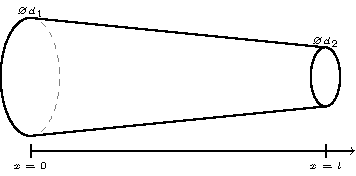
\includegraphics[width = \CaptionWidth]{fig-ex-tikzpicture}
\end{minipage}
\SourceOrNote{adaptada de \textcite{Magdowski2012}}
\end{figure}

Outros exemplos deste tipo de ilustração são apresentados nas \Cref{fig:subfig,fig:ex-uml}.

\subsubsection{Subfiguras}%
\label{sssect:subfig}

É possível produzir subfiguras e imprimir suas respectivas legendas a partir de comandos definidos na classe \texttt{\ifbool{MakeGly}{\gly*{memoir}}{memoir}}:

\begin{snugshade}
\begin{Verbatim}
\subtop[Subtitle\label{Label}]{Subfigure}%   % Acima da subfigura
\subbottom[Subtitle\label{Label}]{Subfigure}%% Abaixo da subfigura
\end{Verbatim}
\end{snugshade}

Além disso, é possível rotular e referenciar as mesmas, por exemplo, as \Cref{sfig:subfig-a,sfig:subfig-b,sfig:subfig-c,sfig:subfig-d,sfig:subfig-e} são exemplos de subfiguras da \Cref{fig:subfig}.

\begin{figure}[!htbp]
\SetCaptionWidth{\textwidth}
\caption{Segundo exemplo de figura, contendo cinco subfiguras}%
\label{fig:subfig}
\subbottom[Primeira subfigura\label{sfig:subfig-a}]{%
  \includegraphics[width = 0.3\CaptionWidth, page = 1]{example-movie}%
}%
\hspace*{0.05\CaptionWidth}%
\subbottom[Segunda subfigura\label{sfig:subfig-b}]{%
  \includegraphics[width = 0.3\CaptionWidth, page = 16]{example-movie}%
}%
\hspace*{0.05\CaptionWidth}%
\subbottom[Terceira subfigura\label{sfig:subfig-c}]{%
  \includegraphics[width = 0.3\CaptionWidth, page = 31]{example-movie}%
}%
\\%
\subbottom[Quarta subfigura\label{sfig:subfig-d}]{%
  \includegraphics[width = 0.3\CaptionWidth, page = 46]{example-movie}%
}%
\hspace*{0.05\CaptionWidth}%
\subbottom[Quinta subfigura\label{sfig:subfig-e}]{%
  \includegraphics[width = 0.3\CaptionWidth, page = 61]{example-movie}%
}%
\SourceOrNote{\textcite{Scharrer2018}}
\end{figure}

Sublegendas do tipo \labelcref{sfig:subfig-a,sfig:subfig-b,sfig:subfig-c,sfig:subfig-d,sfig:subfig-e} podem ser utilizadas também nos demais ambientes de ilustrações, assim como nos ambientes de algoritmos e de tabelas, a partir dos comandos da classe \texttt{\ifbool{MakeGly}{\gly*{memoir}}{memoir}} mostrados no início desta seção.

\subsection{Fluxogramas}%
\label{ssect:fcht}

O \Cref{fcht:ex-algorithms} é um dos vários exemplos deste tipo de ilustração que pode ser produzido ou editado na ferramenta \ENLang{\href{https://www.lucidchart.com/}{Lucidchart\LinkIcon}}.
Outras ferramentas \ENLang{online} podem ser usadas, por exemplo, \href{https://www.drawio.com}{draw.io\LinkIcon}; ou ainda, diversos aplicativos específicos para esta finalidade, por exemplo, \href{http://dia-installer.de/}{Dia\LinkIcon}.

\begin{flowchart}[!htbp]
\SetCaptionWidth{\textwidth}
\caption{Exemplo de fluxograma: \Cref{alg:ex-1,alg:ex-2}}%
\label{fcht:ex-algorithms}
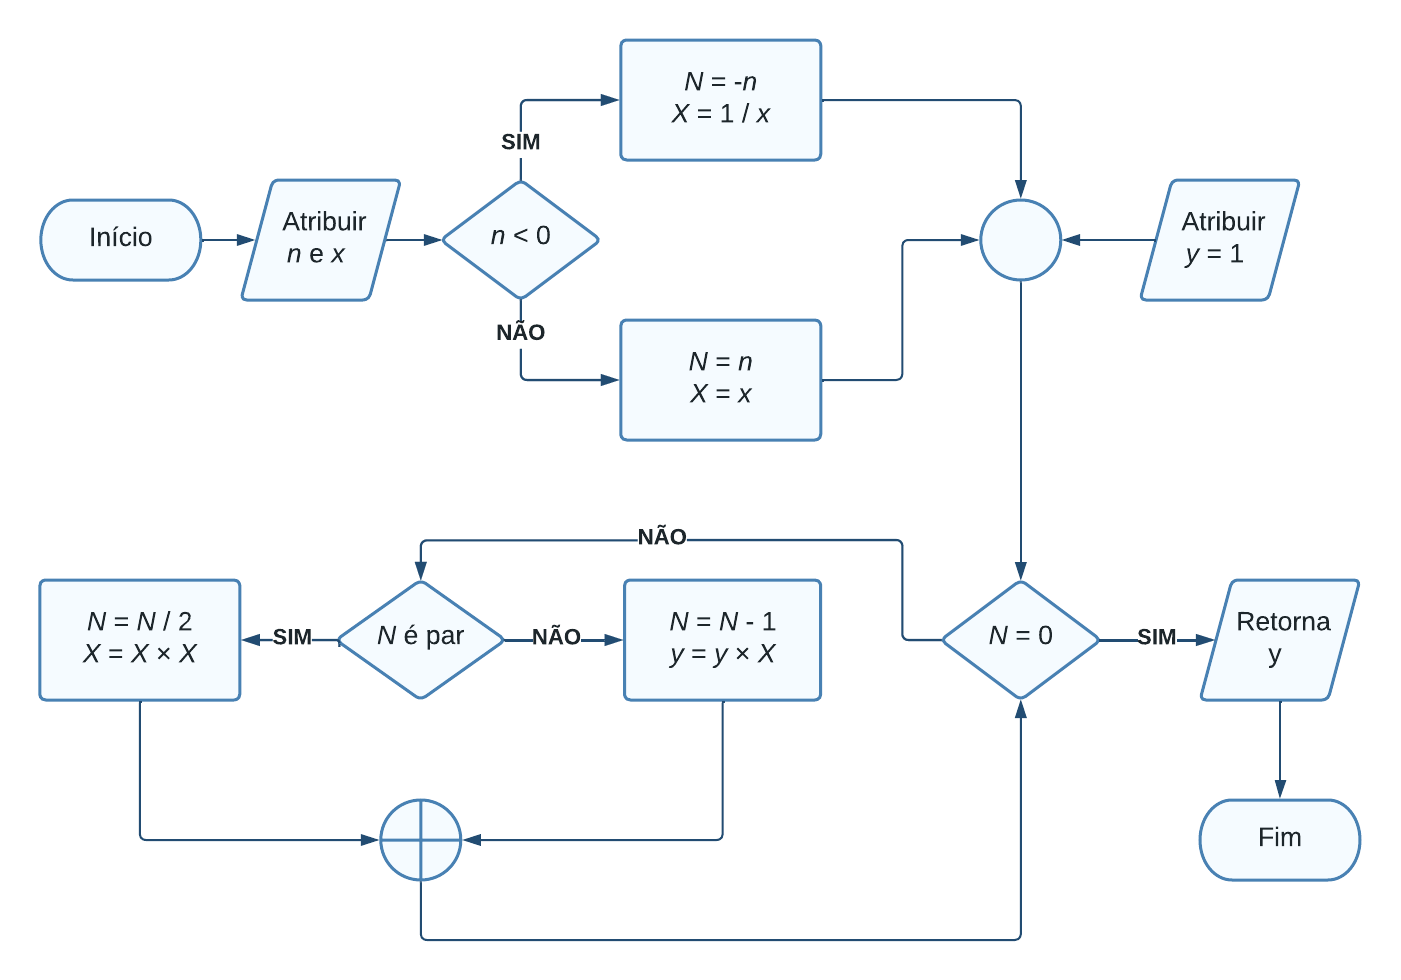
\includegraphics[width = \CaptionWidth]{fcht-ex-algorithms}
\SourceOrNote{autoria própria (\YearNum)}
\end{flowchart}

\subsection{Fotografias}%
\label{ssect:phot}

Um exemplo deste tipo de ilustração é apresentado na \Cref{phot:pg-campus}.

\begin{photograph}[!htbp]
\SetCaptionWidth{0.7\textwidth}
\caption[%
  Fachada do campus Ponta Grossa da UTFPR%
]{%
  Fachada do campus Ponta Grossa da \ifbool{MakeAcr}{\intl{UTFPR}}{UTFPR}%
}%
\label{phot:pg-campus}
\savebox0{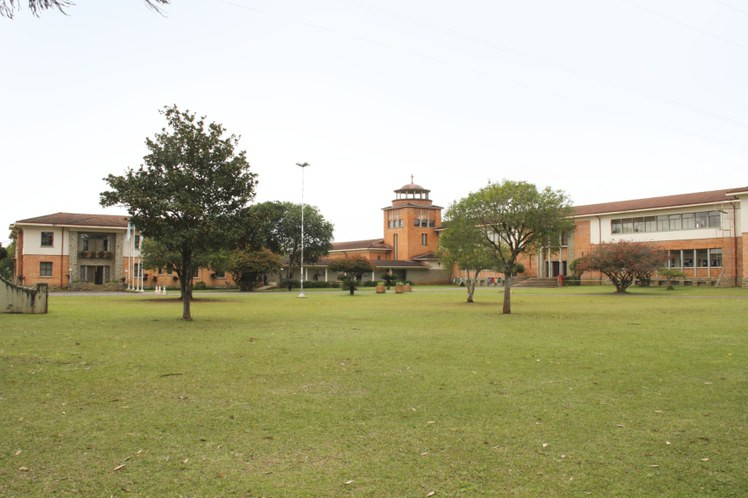
\includegraphics[width = \CaptionWidth]{phot-pg-campus}}
\usebox0%
\llap{%
  \raisebox{\ht0-\height}{%
    \href{https://www.utfpr.edu.br/campus/pontagrossa}{%
      
\includegraphics[height = 15mm]{phot-pg-campus-qr-code}%
    }%
  }%
}
\SourceOrNote{\textcite{UTFPR2018}}
\end{photograph}

Outro exemplo deste tipo de ilustração é apresentado na \Cref{phot:galunggung}.

\begin{photograph}[!htbp]
\SetCaptionWidth{0.7\textwidth}
\caption{Erupção vulcânica em 1982 do Galunggung (com descargas de raios) na Indonésia (foto de pesquisa realizada pelo Serviço Geológico dos Estados Unidos da América)}%
\label{phot:galunggung}
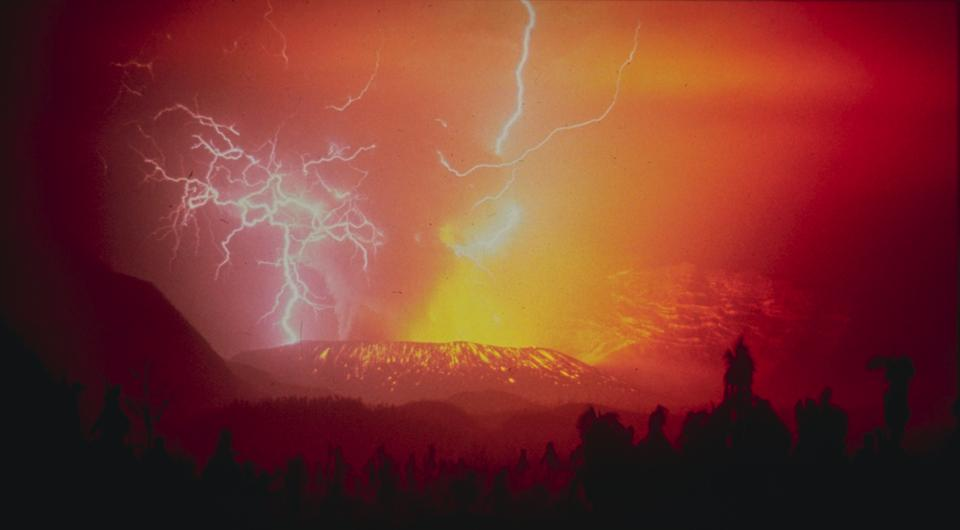
\includegraphics[width = \CaptionWidth]{phot-galunggung}%
\llap{%
  \href{https://en.wikipedia.org/wiki/Galunggung}{%
    
\includegraphics[height = 15mm]{phot-galunggung-qr-code}%
  }%
}
\SourceOrNote{\textcite{Hadian1982}}
\end{photograph}

Como mostrado nas \Cref{phot:pg-campus,phot:galunggung}, objetos flutuantes (ilustrações) podem adicionalmente receber um código de \ifbool{MakeAcr}{\intldescr{QR} (\intldescr+{QR} \textemdash\ \intl{QR})}{Resposta Rápida (\ENLang*{Quick Response} \textemdash\ QR)} contendo: \ifbool{MakeAcr}{\intldescr{URL} (\intldescr+{URL} \textemdash\ \intl{URL})}{Localizador Uniforme de Recursos (\ENLang*{Uniform Resource Locator} \textemdash\ URL)} ou informações complementares.

\subsection{Gráficos}%
\label{ssect:grph}

O ambiente \texttt{minipage} pode ser usado para inserir textos e outros elementos em caixas com tamanhos e posições controladas, conforme exemplos nos \Cref{grph:chi-beta,grph:t-x}, obtidos a partir dos arquivos-fonte \texttt{grph-chi-beta.tex} (\texttt{picture}) e \texttt{grph-t-x.tex} (\texttt{tikzpicture}) em \texttt{./Chapter-Example/Illustrations/}.

\begin{graph}[!htbp]
\begin{minipage}[t]{7cm}
\centering%
\SetCaptionWidth{\linewidth}
\caption{Primeiro exemplo de gráfico em ambiente \texttt{minipage}}%
\label{grph:chi-beta}
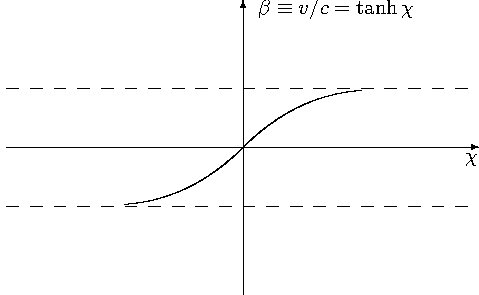
\includegraphics[width = \CaptionWidth]{grph-chi-beta}
\SourceOrNote{autoria própria (\YearNum)}
\end{minipage}
\hfill
\begin{minipage}[t]{8cm}
\centering%
\SetCaptionWidth{\linewidth}
\caption{Segundo exemplo de gráfico em ambiente \texttt{minipage}}%
\label{grph:t-x}
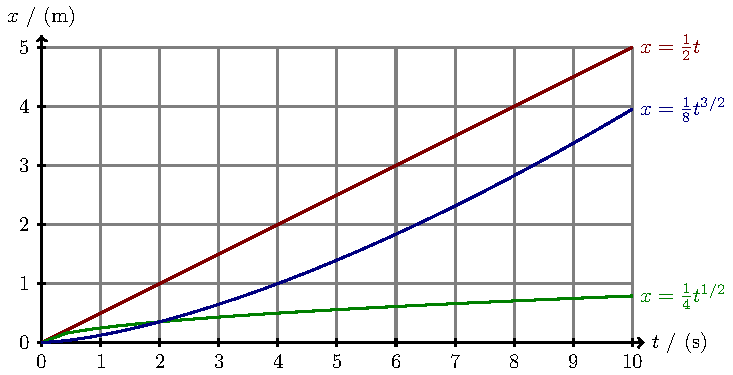
\includegraphics[width = \CaptionWidth]{grph-t-x}
\SourceOrNote{autoria própria (\YearNum)}
\end{minipage}
\end{graph}

Outro exemplo deste tipo de ilustração é apresentado no \Cref{grph:ex-gnuplot}.

\subsection{Quadros}%
\label{ssect:tfrm}

Quadros não devem ser chamados tabelas, visto que se diferenciam destas por apresentarem as laterais fechadas e o conteúdo não numérico, ou seja, são usados para dados qualitativos, predominantemente preenchidos com informações textuais (palavras).
Para quadros que ocupam mais de uma folha, não é necessária nenhuma sinalização.
Exemplos deste tipo de ilustração são apresentados nos \Cref{tfrm:acr-cmd,tfrm:sym-cmd,tfrm:math}.


%% Tabelas
% \section{Tabelas}%
\label{sect:tab}

Diferentemente de quadros, tabelas são usadas para dados quantitativos, predominantemente preenchidos com informações numéricas e sem as laterais fechadas, conforme o \textcite{IBGE1993}.
Tabelas podem ser inseridas no documento usando o ambiente \texttt{table}, conforme exemplos em arquivos-fonte deste modelo.
Sendo assim, a \Cref{tab:ex-1} foi produzida usando este tipo de ambiente.

\begin{table}[!htbp]
\SetCaptionWidth{\textwidth}
\caption{Primeiro exemplo de tabela, com legenda contendo um texto muito longo que pode ocupar mais de uma linha}%
\label{tab:ex-1}
\begin{tabularx}{\CaptionWidth}{e{}@{}l*{4}{,{}}@{}}
\toprule%
\multicolumn{1}{@{}c}{\textbf{Caixa de}}                 &
\multicolumn{1}{c}{\textbf{Aresta, \MathBF{L}}}          &
\multicolumn{1}{c}{\textbf{Altura, \MathBF{H}}}          &
\multicolumn{1}{c}{\textbf{Área, \MathBF{L^2}}}          &
\multicolumn{1}{c@{}}{\textbf{Volume, \MathBF{L^2 H}}}   \\
\multicolumn{1}{@{}c}{\textbf{base quadrada}}            &
\multicolumn{1}{c}{\MathBF{\Unit{\left(cm\right)}}}      &
\multicolumn{1}{c}{\MathBF{\Unit{\left(cm\right)}}}      &
\multicolumn{1}{c}{\MathBF{\Unit{\left(cm^2\right)}}}    &
\multicolumn{1}{c@{}}{\MathBF{\Unit{\left(cm^3\right)}}} \\ \midrule%
A & 1 & 5 & 1  & 5  \\
B & 2 & 4 & 4  & 16 \\
C & 3 & 3 & 9  & 27 \\
D & 4 & 2 & 16 & 32 \\
E & 5 & 1 & 25 & 25 \\ \bottomrule%
\end{tabularx}
\SourceOrNote{autoria própria (\YearNum)}
\end{table}

A \Cref{tab:psbl-trpl} é um exemplo de tabela que ocupa mais de uma página, produzida usando o ambiente \texttt{longtable} do pacote de mesmo nome.
Em cada página, repetem-se a legenda e o cabeçalho; somente na última inserem-se a linha de fechamento e a fonte.
\Citation[brazilian]{\cite[\ifbool{MakeAcr}{\Abrv{sec}}{Seç.} 8.3 \ppno~29]{IBGE1993}}{Cada página deve ter uma das seguintes indicações: continua para a primeira, conclusão para a última e continuação para as demais}.

\begin{longtable}{e{}@{},{}*{2}{c}@{}}
%% Cabeçalho da primeira página
\caption{Possíveis tríplices para grade altamente variável}%
\label{tab:psbl-trpl}                                         \\[\belowcaptionskip]
\multicolumn{3}{@{}r@{}}{\textbf{(continua)}}                 \\[\belowcaptionskip]
\toprule%
\multicolumn{1}{@{}c}{\textbf{Tempo (s)}}                     &
\multicolumn{1}{c}{\textbf{Tríplice escolhida}}               &
\multicolumn{1}{c@{}}{\textbf{Outras possíveis tríplices}}    \\ \midrule%
\endfirsthead%
%% Cabeçalho das páginas (exceto primeira e última)
\caption[]{Possíveis tríplices para grade altamente variável} \\[\belowcaptionskip]
\multicolumn{3}{@{}r@{}}{\textbf{(continuação)}}              \\[\belowcaptionskip]
\toprule%
\multicolumn{1}{@{}c}{\textbf{Tempo (s)}}                     &
\multicolumn{1}{c}{\textbf{Tríplice escolhida}}               &
\multicolumn{1}{c@{}}{\textbf{Outras possíveis tríplices}}    \\ \midrule%
\endhead%
%% Cabeçalho da última página
\caption[]{Possíveis tríplices para grade altamente variável} \\[\belowcaptionskip]
\multicolumn{3}{@{}r@{}}{\textbf{(conclusão)}}                \\[\belowcaptionskip]
\toprule%
\multicolumn{1}{@{}c}{\textbf{Tempo (s)}}                     &
\multicolumn{1}{c}{\textbf{Tríplice escolhida}}               &
\multicolumn{1}{c@{}}{\textbf{Outras possíveis tríplices}}    \\ \midrule%
\endlasthead%
%% Rodapé da última página
\bottomrule%
\LTSourceOrNote{adaptada de \textcite{Smallen2014}}           \\
\endlastfoot%
0      & (1, 11, 13725) & (1, 12, 10980), (1, 13, 8235), (2, 2, 0), (3, 1, 0) \\
2745   & (1, 12, 10980) & (1, 13, 8235), (2, 2, 0), (2, 3, 0), (3, 1, 0)      \\
5490   & (1, 12, 13725) & (2, 2, 2745), (2, 3, 0), (3, 1, 0)                  \\
8235   & (1, 12, 16470) & (1, 13, 13725), (2, 2, 2745), (2, 3, 0), (3, 1, 0)  \\
10980  & (1, 12, 16470) & (1, 13, 13725), (2, 2, 2745), (2, 3, 0), (3, 1, 0)  \\
13725  & (1, 12, 16470) & (1, 13, 13725), (2, 2, 2745), (2, 3, 0), (3, 1, 0)  \\
16470  & (1, 13, 16470) & (2, 2, 2745), (2, 3, 0), (3, 1, 0)                  \\
19215  & (1, 12, 16470) & (1, 13, 13725), (2, 2, 2745), (2, 3, 0), (3, 1, 0)  \\
21960  & (1, 12, 16470) & (1, 13, 13725), (2, 2, 2745), (2, 3, 0), (3, 1, 0)  \\
24705  & (1, 12, 16470) & (1, 13, 13725), (2, 2, 2745), (2, 3, 0), (3, 1, 0)  \\
27450  & (1, 12, 16470) & (1, 13, 13725), (2, 2, 2745), (2, 3, 0), (3, 1, 0)  \\
30195  & (2, 2, 2745)   & (2, 3, 0), (3, 1, 0)                                \\
32940  & (1, 13, 16470) & (2, 2, 2745), (2, 3, 0), (3, 1, 0)                  \\
35685  & (1, 13, 13725) & (2, 2, 2745), (2, 3, 0), (3, 1, 0)                  \\
38430  & (1, 13, 10980) & (2, 2, 2745), (2, 3, 0), (3, 1, 0)                  \\
41175  & (1, 12, 13725) & (1, 13, 10980), (2, 2, 2745), (2, 3, 0), (3, 1, 0)  \\
43920  & (1, 13, 10980) & (2, 2, 2745), (2, 3, 0), (3, 1, 0)                  \\
46665  & (2, 2, 2745)   & (2, 3, 0), (3, 1, 0)                                \\
49410  & (2, 2, 2745)   & (2, 3, 0), (3, 1, 0)                                \\
52155  & (1, 12, 16470) & (1, 13, 13725), (2, 2, 2745), (2, 3, 0), (3, 1, 0)  \\
54900  & (1, 13, 13725) & (2, 2, 2745), (2, 3, 0), (3, 1, 0)                  \\
57645  & (1, 13, 13725) & (2, 2, 2745), (2, 3, 0), (3, 1, 0)                  \\
60390  & (1, 12, 13725) & (2, 2, 2745), (2, 3, 0), (3, 1, 0)                  \\
63135  & (1, 13, 16470) & (2, 2, 2745), (2, 3, 0), (3, 1, 0)                  \\
65880  & (1, 13, 16470) & (2, 2, 2745), (2, 3, 0), (3, 1, 0)                  \\
68625  & (2, 2, 2745)   & (2, 3, 0), (3, 1, 0)                                \\
71370  & (1, 13, 13725) & (2, 2, 2745), (2, 3, 0), (3, 1, 0)                  \\
74115  & (1, 12, 13725) & (2, 2, 2745), (2, 3, 0), (3, 1, 0)                  \\
76860  & (1, 13, 13725) & (2, 2, 2745), (2, 3, 0), (3, 1, 0)                  \\
79605  & (1, 13, 13725) & (2, 2, 2745), (2, 3, 0), (3, 1, 0)                  \\
82350  & (1, 12, 13725) & (2, 2, 2745), (2, 3, 0), (3, 1, 0)                  \\
85095  & (1, 12, 13725) & (1, 13, 10980), (2, 2, 2745), (2, 3, 0), (3, 1, 0)  \\
87840  & (1, 13, 16470) & (2, 2, 2745), (2, 3, 0), (3, 1, 0)                  \\
90585  & (1, 13, 16470) & (2, 2, 2745), (2, 3, 0), (3, 1, 0)                  \\
93330  & (1, 13, 13725) & (2, 2, 2745), (2, 3, 0), (3, 1, 0)                  \\
96075  & (1, 13, 16470) & (2, 2, 2745), (2, 3, 0), (3, 1, 0)                  \\
98820  & (1, 13, 16470) & (2, 2, 2745), (2, 3, 0), (3, 1, 0)                  \\
101565 & (1, 13, 13725) & (2, 2, 2745), (2, 3, 0), (3, 1, 0)                  \\
104310 & (1, 13, 16470) & (2, 2, 2745), (2, 3, 0), (3, 1, 0)                  \\
107055 & (1, 13, 13725) & (2, 2, 2745), (2, 3, 0), (3, 1, 0)                  \\
109800 & (1, 13, 13725) & (2, 2, 2745), (2, 3, 0), (3, 1, 0)                  \\
112545 & (1, 12, 16470) & (1, 13, 13725), (2, 2, 2745), (2, 3, 0), (3, 1, 0)  \\
115290 & (1, 13, 16470) & (2, 2, 2745), (2, 3, 0), (3, 1, 0)                  \\
118035 & (1, 13, 13725) & (2, 2, 2745), (2, 3, 0), (3, 1, 0)                  \\
120780 & (1, 13, 16470) & (2, 2, 2745), (2, 3, 0), (3, 1, 0)                  \\
123525 & (1, 13, 13725) & (2, 2, 2745), (2, 3, 0), (3, 1, 0)                  \\
126270 & (1, 12, 16470) & (1, 13, 13725), (2, 2, 2745), (2, 3, 0), (3, 1, 0)  \\
129015 & (2, 2, 2745)   & (2, 3, 0), (3, 1, 0)                                \\
131760 & (2, 2, 2745)   & (2, 3, 0), (3, 1, 0)                                \\
134505 & (1, 13, 16470) & (2, 2, 2745), (2, 3, 0), (3, 1, 0)                  \\
137250 & (1, 13, 13725) & (2, 2, 2745), (2, 3, 0), (3, 1, 0)                  \\
139995 & (2, 2, 2745)   & (2, 3, 0), (3, 1, 0)                                \\
142740 & (2, 2, 2745)   & (2, 3, 0), (3, 1, 0)                                \\
145485 & (1, 12, 16470) & (1, 13, 13725), (2, 2, 2745), (2, 3, 0), (3, 1, 0)  \\
148230 & (2, 2, 2745)   & (2, 3, 0), (3, 1, 0)                                \\
150975 & (1, 13, 16470) & (2, 2, 2745), (2, 3, 0), (3, 1, 0)                  \\
153720 & (1, 12, 13725) & (2, 2, 2745), (2, 3, 0), (3, 1, 0)                  \\
156465 & (1, 13, 13725) & (2, 2, 2745), (2, 3, 0), (3, 1, 0)                  \\
159210 & (1, 13, 13725) & (2, 2, 2745), (2, 3, 0), (3, 1, 0)                  \\
161955 & (1, 13, 16470) & (2, 2, 2745), (2, 3, 0), (3, 1, 0)                  \\
164700 & (1, 13, 13725) & (2, 2, 2745), (2, 3, 0), (3, 1, 0)                  \\
\end{longtable}

Diversas ferramentas podem ser usadas para gerar ou editar tabelas, por exemplo: \ENLang{\href{https://www.tablesgenerator.com/}{Tables Generator\LinkIcon} e \href{https://www.latex-tables.com/}{\ifbool{MakeGly}{\gly*{LaTeX}}{\LaTeX} Tables Editor\LinkIcon}}.
Tabelas produzidas em planilhas do Microsoft\textsuperscript{\textregistered} Excel\textsuperscript{\textregistered} podem ser convertidas em tabelas \ifbool{MakeGly}{\gly*{LaTeX}}{\LaTeX} usando o suplemento \href{https://www.ctan.org/pkg/excel2latex}{Excel2\ifbool{MakeGly}{\gly*{LaTeX}}{\LaTeX}\LinkIcon}.
Outro exemplo deste tipo de ilustração é apresentado na \Cref{tab:quot}.


%% Abreviaturas e siglas
% \section{Abreviaturas e siglas}%
\label{sect:acr}

Abreviaturas e siglas podem ser definidas ao longo do texto, preferencialmente antes do seu primeiro uso, ou em um arquivo de entradas.
Tal arquivo pode ser incluído no preâmbulo do principal arquivo-fonte (ver \texttt{./utfpr-thesis.tex}) pelo comando:

\begin{snugshade}
\begin{Verbatim}
\MakeAcronyms[File]%% Por exemplo, acronyms-entries.tex em ./Pre-Textual/Optionals/
\end{Verbatim}
\end{snugshade}

Os termos são definidos usando os comandos do pacote \texttt{utfpr-thesis}:

\begin{snugshade}
\begin{Verbatim}
\New<AcronymType>Entry{Label}{%% Usar somente letras latinas não acentuadas
  Term        = {...},%        % Obrigatório
  Description = {...},%        % Obrigatório
  Plural      = {...},%        % Opcional
  Translation = {...},%        % Opcional (descrição original em inglês)
}
\end{Verbatim}
\end{snugshade}

\noindent Onde \texttt{<AcronymType>} é igual a \texttt{Abbreviation} (abreviatura) ou \texttt{Initials} (sigla).

Para que abreviaturas e siglas sejam impressos em alguma parte do texto do documento e adicionados na \acrref, usam-se os comandos do pacote \texttt{utfpr-thesis} apresentados no \Cref{tfrm:acr-cmd}.
Os comandos com letras em maiúscula imprimem o termo, a descrição e o plural (se definido) com a letra inicial em maiúscula.
Por exemplo, \ColorBox{shadecolor}{\Verb|\abrv{cap}|} e \ColorBox{shadecolor}{\Verb|\Abrv{cap}|} resultam em: \ifbool{MakeAcr}{\abrv{cap} e \Abrv{cap}}{cap.\ e Cap.}, respectivamente.

\begin{tabframed}[!htbp]
\SetCaptionWidth{\textwidth}
\caption{Comandos para impressão de abreviaturas e siglas no texto}%
\label{tfrm:acr-cmd}
\begin{tabularx}{\CaptionWidth}{?{}l*{3}{|>{\columncolor{shadecolor}}Y}?{}}%% CHKTEX 44
\toprule%
\multicolumn{1}{?{}c|}{\textbf{Tipo}}                                &
\multicolumn{1}{Y|}{\textbf{Termo}\rlap{\MathBF{^{(1)}}}}            &
\multicolumn{1}{Y|}{\textbf{Descrição}\rlap{\MathBF{^{{(1)}{(2)}}}}} &
\multicolumn{1}{Y?{}}{\textbf{Plural}\rlap{\MathBF{^{(1)}}}}         \\ \midrule%
Abreviatura & \Verb|\abrv{Label}|                & \Verb|\abrvdescr{Label}|                & \Verb|\abrvpl{Label}|                \\ \cline{2-4}
            & \Verb|\Abrv{Label}|\rlap{$^{(3)}$} & \Verb|\AbrvDescr{Label}|\rlap{$^{(3)}$} & \Verb|\AbrvPl{Label}|\rlap{$^{(3)}$} \\ \midrule%
Sigla       & \Verb|\intl{Label}|                & \Verb|\intldescr{Label}|                & \Verb|\intlpl{Label}|                \\ \cline{2-4}
            & \Verb|\Intl{Label}|\rlap{$^{(3)}$} & \Verb|\IntlDescr{Label}|\rlap{$^{(3)}$} & \Verb|\IntlPl{Label}|\rlap{$^{(3)}$} \\ \bottomrule%
\end{tabularx}
\SourceOrNote{autoria própria (\YearNum)}
\SourceOrNote+*[\MathBF{^{(1)}}][]{Adiciona (automaticamente) também no \protect\idxref\ com um asterisco (*) opcional, por exemplo, \ColorBox{shadecolor}{\protect\Verb|\abrv*{Label}|}}
\SourceOrNote+*[\MathBF{^{(2)}}][]{Imprime a descrição original em inglês (se definida) com um sinal de mais (+) opcional, por exemplo, \ColorBox{shadecolor}{\protect\Verb|\abrvdescr+{Label}|}}
\SourceOrNote+*[\MathBF{^{(3)}}][]{Imprime com a letra inicial em maiúscula}
\end{tabframed}

Alguns exemplos de abreviaturas e siglas:

\begin{itemize}
\item Abreviaturas: \ifbool{MakeAcr}{\abrvdescr*{1D} (\abrv*{1D}; no plural, \abrvpl*{1D}), \abrvdescr*{art} (\abrv*{art}; no plural, \abrvpl*{art}), \abrvdescr{cap}\phantomsection\label{err:chpt-5} (\abrv{cap}; no plural, \abrvpl{cap}) e \abrvdescr{sec} (\abrv{sec}; no plural, \abrvpl{sec})}{unidimensional (1D\@; no plural, 1Ds), artigo (art.; no plural, arts.), capítulo\phantomsection\label{err:chpt-5} (cap.; no plural, caps.) e seção (seç.; no plural, seçs.)}.
\item Siglas: \ifbool{MakeAcr}{\intldescr{CAPES} (\intl{CAPES}), \intldescr{CNPq} (\intl{CNPq}) e \intldescr{GNU} (\intldescr+{GNU} \textemdash\ \intl{GNU})}{Coordenação de Aperfeiçoamento de Pessoal de Nível Superior (CAPES), Conselho Nacional de Desenvolvimento Científico e Tecnológico (CNPq) e GNU Não é Unix (\ENLang*{GNU is Not Unix} \textemdash\ GNU)}.
\end{itemize}


%% Símbolos
% \section{Símbolos}%
\label{sect:sym}

Símbolos devem ser definidos ao longo do texto antes do seu primeiro uso, ou em um arquivo de entradas.
Tal arquivo pode ser incluído no preâmbulo do principal arquivo-fonte (ver \texttt{./utfpr-thesis.tex}) pelo comando:

\begin{snugshade}
\begin{Verbatim}
\MakeSymbols[File]%% Por exemplo, symbols-entries.tex em ./Pre-Textual/Optionals/
\end{Verbatim}
\end{snugshade}

Os termos são definidos usando os comandos do pacote \texttt{utfpr-thesis}:

\begin{snugshade}
\begin{Verbatim}
\New<SymbolType>Entry{Label}{%% Usar somente letras latinas não acentuadas
  Term        = {...},%       % Obrigatório
  Description = {...},%       % Obrigatório
  Unit        = {...},%       % Opcional
  Sort        = {...},%       % Opcional (para reordenar na lista)
}
\end{Verbatim}
\end{snugshade}

\noindent Onde \texttt{<SymbolType>} é igual a \texttt{Notation} (notação), \texttt{Superscript} (sobrescrito), \texttt{Subscript} (subscrito), \texttt{GreekLetter} (letra grega) ou \texttt{LatinLetter} (letra latina).

Para que símbolos sejam impressos em alguma parte do texto do documento e adicionados na \symref, usam-se os comandos do pacote \texttt{utfpr-thesis} apresentados no \Cref{tfrm:sym-cmd}.
Os comandos de descrição com letras em maiúsculas imprimem a descrição com a letra inicial em maiúscula.
Por exemplo, \ColorBox{shadecolor}{\Verb|\ltnldescr{A}|} e \ColorBox{shadecolor}{\Verb|\LtnLDescr{A}|} resultam em: \ifbool{MakeSym}{\ltnldescr{A} e \LtnLDescr{A}}{área e Área}, respectivamente.

\begin{tabframed}[!htbp]
\SetCaptionWidth{\textwidth}
\caption{Comandos para impressão de símbolos no texto}%
\label{tfrm:sym-cmd}
\begin{tabularx}{\CaptionWidth}{?{}l*{3}{|>{\columncolor{shadecolor}}Y}?{}}%% CHKTEX 44
\toprule%
\multicolumn{1}{?{}c|}{\textbf{Tipo}}                         &
\multicolumn{1}{Y|}{\textbf{Termo}\rlap{\MathBF{^{(1)}}}}     &
\multicolumn{1}{Y|}{\textbf{Descrição}\rlap{\MathBF{^{(1)}}}} &
\multicolumn{1}{Y?{}}{\textbf{Unidade}}                       \\ \midrule%
Notação      & \Verb|\nttn{Label}|\rlap{$^{(2)}$} & \Verb|\nttndescr{Label}|                & \Verb|\nttnunit{Label}| \\ \cline{2-4}
             & {\textendash}                      & \Verb|\NttnDescr{Label}|\rlap{$^{(3)}$} & {\textendash}           \\ \midrule%
Sobrescrito  & \Verb|\sprs{Label}|                & \Verb|\sprsdescr{Label}|                & \Verb|\sprsunit{Label}| \\ \cline{2-4}
             & {\textendash}                      & \Verb|\SprsDescr{Label}|\rlap{$^{(3)}$} & {\textendash}           \\ \midrule%
Subscrito    & \Verb|\sbsc{Label}|                & \Verb|\sbscdescr{Label}|                & \Verb|\sbscunit{Label}| \\ \cline{2-4}
             & {\textendash}                      & \Verb|\SbscDescr{Label}|\rlap{$^{(3)}$} & {\textendash}           \\ \midrule%
Letra grega  & \Verb|\grkl{Label}|                & \Verb|\grkldescr{Label}|                & \Verb|\grklunit{Label}| \\ \cline{2-4}
             & {\textendash}                      & \Verb|\GrkLDescr{Label}|\rlap{$^{(3)}$} & {\textendash}           \\ \midrule%
Letra latina & \Verb|\ltnl{Label}|                & \Verb|\ltnldescr{Label}|                & \Verb|\ltnlunit{Label}| \\ \cline{2-4}
             & {\textendash}                      & \Verb|\LtnLDescr{Label}|\rlap{$^{(3)}$} & {\textendash}           \\ \bottomrule%
\end{tabularx}
\SourceOrNote{autoria própria (\YearNum)}
\SourceOrNote+*[\MathBF{^{(1)}}][]{Adiciona (automaticamente) também no \protect\idxref\ com um asterisco (*) opcional, por exemplo, \ColorBox{shadecolor}{\protect\Verb|\nttn*{Label}|}}
\SourceOrNote+*[\MathBF{^{(2)}}][]{Armazena um símbolo no comando \ColorBox{shadecolor}{\protect\Verb|\MrkSym|} (o caractere tipográfico \DottedCircle\ por padrão, no qual se aplica a notação durante a impressão da mesma) com um segundo argumento (opcional: {\ColorBox{shadecolor}{\protect\Verb|\nttn{Label}[MrkSym]|}})}
\SourceOrNote+*[\MathBF{^{(3)}}][]{Imprime com a letra inicial em maiúscula}
\end{tabframed}

Alguns exemplos de símbolos:

\begin{itemize}
\item Notações: \ifbool{MakeSym}{\nttn{averagea} representa a \nttndescr{averagea}, \nttn{averageb} representa a \nttndescr{averageb} e \nttn*{gradient} representa o \nttndescr*{gradient}}{$\overline{\MrkSym}$ representa a média temporal, $\langle\MrkSym\rangle$ representa a média na seção transversal e $\vec{\nabla}$ representa o operador gradiente}.
\item Sobrescritos: \ifbool{MakeSym}{\MrkSym\sprs{minus} representa o \sprsdescr{minus}, \MrkSym\sprs{plus} representa o \sprsdescr{plus} e \MrkSym\sprs*{zero} representa o \sprsdescr*{zero}}{$\MrkSym^-$ representa o passo de tempo anterior, $\MrkSym^+$ representa o passo de tempo posterior e $\MrkSym^0$ representa o valor inicial}.
\item Subscritos: \ifbool{MakeSym}{\MrkSym\sbsc{G} representa a \sbscdescr{G}, \MrkSym\sbsc{L} representa a \sbscdescr{L} e \MrkSym\sbsc*{S} representa a \sbscdescr*{S}}{$\MrkSym_\mathrm{G}$ representa a fase gasosa, $\MrkSym_\mathrm{L}$ representa a fase líquida e $\MrkSym_\mathrm{S}$ representa a fase sólida}.
\item Letras gregas: \ifbool{MakeSym}{\grkl{mu} é a \grkldescr{mu} [\grklunit{mu}], \grkl{nu} é a \grkldescr{nu} (\grklunit{nu}), \grkl{pi} é a \grkldescr{pi} (\grklunit{pi}), \grkl{rho} é a \grkldescr{rho} (\grklunit{rho}) e \grkl*{theta} é a \grkldescr*{theta} (\grklunit{theta})}{$\mu$ é a viscosidade dinâmica [\Unit{kg/{(m{\cdot}s)}}], $\nu$ é a viscosidade cinemática (\Unit{m^2/s}), $\pi$ é a constante circular (\Unit{rad}), $\rho$ é a massa específica (\Unit{kg/m^3}) e $\theta$ é a inclinação (\Unit{\Degree})}.
\item Letras latinas: \ifbool{MakeSym}{\ltnl{A} é a \ltnldescr{A} (\ltnlunit{A}), \ltnl{D} é o \ltnldescr{D} (\ltnlunit{D}), \ltnl{L} é o \ltnldescr{L} (\ltnlunit{L}), \ltnl{R} é o \ltnldescr{R} (\ltnlunit{R}), \ltnl*{Re} é o \ltnldescr*{Re} e \ltnl*{V} é a \ltnldescr*{V} (\ltnlunit{V})}{$A$ é a área (\Unit{m^2}), $D$ é o diâmetro (\Unit{m}), $L$ é o comprimento (\Unit{m}), $R$ é o raio (\Unit{m}), $\mathrm{Re}$ é o número de Reynolds e $V$ é a velocidade (\Unit{m/s})}.
\end{itemize}

Os símbolos de quantidades (grandezas) e unidades devem ser expressos conforme \textcite{Inmetro2021}.


%% Referências
% \section{Referências}%
\label{sect:ref}

A formatação das \refref\ conforme a \textcite[\ifbool{MakeAcr}{\intl{NBR}}{NBR} 6023]{ABNT2018NBR6023} é um dos principais objetivos deste modelo\footnote{\href{https://github.com/abntex/biblatex-abnt/issues/42}{Modificações da norma vigente\LinkIcon} devem estar em uma versão $\ge$ 3.5 do \href{https://ctan.org/pkg/biblatex-abnt}{\ifbool{MakeGly}{\gly*{BibLaTeXabnt}}{Bib\LaTeX-abnt}\LinkIcon}}.
Isto é feito usando os pacotes \href{https://ctan.org/pkg/biblatex}{\ifbool{MakeGly}{\gly*{BibLaTeX}}{Bib\LaTeX}\LinkIcon} e \href{https://ctan.org/pkg/biblatex-abnt}{\ifbool{MakeGly}{\gly*{BibLaTeXabnt}}{Bib\LaTeX-abnt}\LinkIcon}, cujos manuais fornecem informações sobre configuração e utilização.

\ifbool{MakeGly}{\gly*{LaTeX}}{\LaTeX} pode usar arquivos de banco de dados (entradas) das \refref\ citadas no texto, geralmente obtidos na própria página de acesso ou \ENLang{download} da publicação (artigos, livros, etc.) ou, ainda, a partir do Google Acadêmico, etc.
Estes arquivos (\texttt{*.bib}) são compilados pelo \ifbool{MakeGly}{\gly*{BibTeX}}{Bib\TeX} (ou \ifbool{MakeGly}{\gly*{biber}}{biber} por padrão, no caso do \href{https://ctan.org/pkg/biblatex}{\ifbool{MakeGly}{\gly*{BibLaTeX}}{Bib\LaTeX}\LinkIcon}), como os arquivos \texttt{references.bib} e \texttt{references-examples.bib} presentes em \texttt{./Post-Textual/}.
Diversas ferramentas podem ser usadas para gerar ou editar entradas de tais arquivos, por exemplo: \ENLang{\href{https://zbib.org/}{ZoteroBib\LinkIcon} e \href{https://truben.no/latex/bibtex/}{\ifbool{MakeGly}{\gly*{BibTeX}}{Bib\TeX} Editor\LinkIcon}}.
Além disso, há alguns aplicativos para gerenciamento de \refref, como \href{https://www.jabref.org/}{JabRef\LinkIcon}.

\subsection{Acentuação em referências}%
\label{ssect:accnt-ref}

Normalmente, não há problemas em usar caracteres acentuados em arquivos de base bibliográfica (extensão \texttt{bib}).
Contudo, como as regras da \ifbool{MakeAcr}{\intl{ABNT}}{ABNT} fazem uso quase abusivo da conversão para letras em maiúsculas, é preciso observar o modo como se escreve os nomes dos autores e editores.
A regra geral é sempre usar as conversões de acentuação quando houver conversão para letras em maiúsculas, especialmente se estiver compilando com o \ifbool{MakeGly}{\gly*{BibTeX}}{Bib\TeX}.
No caso de compilação com \ifbool{MakeGly}{\gly*{biber}}{biber}, padrão do \href{https://ctan.org/pkg/biblatex}{\ifbool{MakeGly}{\gly*{BibLaTeX}}{Bib\LaTeX}\LinkIcon}, estas conversões de acentuação são desnecessárias, visto que o \ifbool{MakeGly}{\gly*{biber}}{biber} já converte automaticamente caracteres em \ifbool{MakeAcr}{\intl{UTF8}}{UTF-8}, inclusive do \ifbool{MakeGly}{\gly*{LaTeX}}{\LaTeX}.
Informações sobre caracteres especiais e conversões de acentuação podem ser observadas em \url{https://en.wikibooks.org/wiki/LaTeX/Special_Characters}.


%% Glossário
% \section{Glossário}%
\label{sect:gly}

Termos de \glyref\ podem ser definidos ao longo do texto, preferencialmente antes do seu primeiro uso, ou em um arquivo de entradas.
Tal arquivo pode ser incluído no preâmbulo do principal arquivo-fonte (ver \texttt{./utfpr-thesis.tex}) pelo comando:

\begin{snugshade}
\begin{Verbatim}
\MakeGlossary[File]%% Por exemplo, glossary-entries.tex em ./Post-Textual/Optionals/
\end{Verbatim}
\end{snugshade}

Os termos são definidos usando o comando do pacote \texttt{utfpr-thesis}:

\begin{snugshade}
\begin{Verbatim}
\NewGlossaryEntry{Label}{%% Usar somente letras latinas não acentuadas
  Term        = {...},%   % Obrigatório
  Description = {...},%   % Obrigatório
  Plural      = {...},%   % Opcional
  Parent      = {...},%   % Opcional
}
\end{Verbatim}
\end{snugshade}

\noindent Observação: se a letra inicial do termo, da descrição ou do plural for acentuada, deve ser colocada entre chaves, por exemplo, \ColorBox{shadecolor}{\texttt{Description = \{\{á\}rea\}}}.
Isto se aplica também para abreviaturas e siglas e para símbolos (exceto termo e plural para este último).

Para que termos de \glyref\ sejam impressos em alguma parte do texto do documento (e, consequentemente, sejam adicionados no \glyref), usam-se os comandos do pacote \texttt{utfpr-thesis}:

\begin{snugshade}
\begin{Verbatim}
\gly{Label}%     % Termo
\Gly{Label}%     % Termo com letra inicial em maiúscula
\glydescr{Label}%% Descrição
\GlyDescr{Label}%% Descrição com letra inicial em maiúscula
\glypl{Label}%   % Plural
\GlyPl{Label}%   % Plural com letra inicial em maiúscula
\end{Verbatim}
\end{snugshade}

\noindent Os comandos com letra inicial em maiúscula imprimem o termo, a descrição e o plural (se definido) com a letra inicial em maiúscula.
As versões destes comandos com um asterisco (*) opcional, por exemplo, \ColorBox{shadecolor}{\Verb|\gly*{Label}|}, adicionam o termo também no \idxref, exceto os comandos de descrição.
Seguem alguns exemplos.

\enquote{\ifbool{MakeGly}{\gly*{UTFPRThesis} é um \glydescr{UTFPRThesis}}{\UTFPR-Thesis é um modelo \LaTeX\ que permite atender os requisitos das normas definidas pela UTFPR para elaboração de trabalhos acadêmicos}}.
Esta citação direta curta corresponde a um exemplo de termo definido no \glyref\ e usado no decorrer do texto, assim como:

\begin{DisplayCitation}[brazilian]{}
Esta frase usa a palavra \ifbool{MakeGly}{\gly*{componente}}{componente} e o plural \ifbool{MakeGly}{\glypl*{filho}}{filhos}, ambas definidas no \glyref\ como filhas da entrada \ifbool{MakeGly}{\gly*{pai}}{pai}.
\ifbool{MakeGly}{\Gly*{equilibriodaconfiguracao}}{Equilíbrio da configuração} exemplifica o uso de um termo no início de uma frase.
O modelo \ifbool{MakeGly}{\gly*{UTFPRThesis}}{\UTFPR-Thesis} é escrito em \ifbool{MakeGly}{\gly*{LaTeX}}{\LaTeX}, definido no \glyref\ como \enquote{\ifbool{MakeGly}{\glydescr{LaTeX}}{conjunto de macros para o processador de textos \TeX, utilizado amplamente para a produção de textos matemáticos e científicos devido à sua alta qualidade tipográfica}}.
\end{DisplayCitation}

O texto desta \Index{citação} \Index[citação]{direta} longa foi produzido com:

\begin{snugshade}
\begin{Verbatim}[numbers = left]
\begin{DisplayCitation}[brazilian]{}
Esta frase usa a palavra \ifbool{MakeGly}{\gly*{componente}}{componente} e o plural \ifbool{MakeGly}{\glypl*{filho}}{filhos}, ambas definidas no \glyref\ como filhas da entrada \ifbool{MakeGly}{\gly*{pai}}{pai}.
\ifbool{MakeGly}{\Gly*{equilibriodaconfiguracao}}{Equilíbrio da configuração} exemplifica o uso de um termo no início de uma frase.
O modelo \ifbool{MakeGly}{\gly*{UTFPRThesis}}{\UTFPR-Thesis} é escrito em \ifbool{MakeGly}{\gly*{LaTeX}}{\LaTeX}, definido no \glyref\ como \enquote{\ifbool{MakeGly}{\glydescr{LaTeX}}{conjunto de macros para o processador de textos \TeX, utilizado amplamente para a produção de textos matemáticos e científicos devido à sua alta qualidade tipográfica}}.
\end{DisplayCitation}
\end{Verbatim}
\end{snugshade}


%% Apêndices e Anexos
% \section{Apêndices e anexos}%
\label{sect:apx-anx}

O comando \ColorBox{shadecolor}{\Verb|\appendix|} faz com que todos os capítulos\phantomsection\label{err:chpt-6} subsequentes sejam considerados e formatados como \apxsref.
Neste modelo, os mesmos podem ser inseridos no ambiente \texttt{Appendices} para produzir \apxsref, ou ainda no ambiente \texttt{Annexes}, para produzir \anxsref, ambos do pacote \texttt{utfpr-thesis}.
Os comandos \ColorBox{shadecolor}{\Verb|\AppendicesPart|} e \ColorBox{shadecolor}{\Verb|\AnnexesPart|} produzem as folhas separadoras (similar ao comando \ColorBox{shadecolor}{\Verb|\part|}) denominadas \apxsref\ e \anxsref, respectivamente.

\apxsref\ e \anxsref\ podem ser inseridos no documento, logo após o \glyref, por meio da inclusão de arquivos.
Ver orientações sobre inclusão de arquivos na \Cref{sect:files-incl}.
Por exemplo, os arquivos-fonte \texttt{appendix-a.tex}, \texttt{appendix-b.tex}, \texttt{annex-a.tex} e \texttt{annex-b.tex}, presentes em \texttt{./Post-Textual/} deste modelo, são usados para produzir os \Cref{chpt:apx-a,chpt:apx-b} e os \Cref{chpt:anx-a,chpt:anx-b}, respectivamente.
É possível dividir os \apxsref\ e \anxsref\ em seções, conforme exemplos:

\begin{itemize}
\item Seção secundária de apêndice (\Cref{sect:apx-a2}).
\item Seção terciária de apêndice (\Cref{ssect:apx-a3}).
\item Seção quaternária de apêndice (\Cref{sssect:apx-a4}).
\item Seção quinária de apêndice (\Cref{prgh:apx-a5}).
\item Parágrafo (divisão de seção quinária) de apêndice (\Cref{sprgh:apx-a6}).
\item Seção secundária de anexo (\Cref{sect:anx-b2}).
\item Seção terciária de anexo (\Cref{ssect:anx-b3}).
\item Seção quaternária de anexo (\Cref{sssect:anx-b4}).
\item Seção quinária de anexo (\Cref{prgh:anx-b5}).
\item Parágrafo (divisão de seção quinária) de anexo (\Cref{sprgh:anx-b6}).
\end{itemize}


%% Índice Remissivo
% \section{Índice remissivo}%
\label{sect:idx}

Palavras ou símbolos são indexados no \idxref\ usando os seguintes comandos:

\begin{snugshade}
\begin{Verbatim}
\index{Header to Index}%                % Padrão do makeindex
\Index{Header to Index}[Header to Sort]%% Definido no pacote utfpr-thesis
\end{Verbatim}
\end{snugshade}

\noindent O primeiro somente indexa (padrão do makeindex\footnote{Ver manual do \href{https://www.ctan.org/pkg/makeindex}{\texttt{makeindex}\LinkIcon} para mais detalhes}) e o segundo indexa e imprime localmente o argumento obrigatório\footnote{O argumento opcional possibilita reordenar no \idxref} (definido no pacote \texttt{utfpr-thesis}).

Para complementação, argumentos opcionais podem ser adicionados antes do obrigatório no segundo comando para indexar em subdivisões (no máximo, mais dois níveis), além de imprimir localmente:

\begin{snugshade}
\begin{Verbatim}
\Index{Header to Index}%                                         % Nível 1
\Index[Indexed Header]{Subheader to Index}%                      % Nível 2
\Index[Indexed Header][Indexed Subheader]{Subsubheader to Index}%% Nível 3
\end{Verbatim}
\end{snugshade}

\noindent Por exemplo: a \Index{casa} possui uma \Index[casa]{porta} de \Index[casa][porta]{madeira} e uma \Index[casa]{janela} de \Index[casa][janela]{metal}.

O pacote \texttt{utfpr-thesis} também fornece comandos para indexar palavras ou símbolos a suas remissivas e imprimi-las localmente:

\begin{snugshade}
\begin{Verbatim}
\IndexSee{Header to Index}{Indexed Remissive}%    % Remissiva ver
\IndexSeeAlso{Header to Index}{Indexed Remissive}%% Remissiva ver também
\end{Verbatim}
\end{snugshade}

\noindent Por exemplo: \Index{rato}-\Index[rato]{doméstico}, \IndexSee{camundongo}{rato} (sinônimo) e \IndexSeeAlso{ratazana}{rato} (termo correlato).


%% Inclusão de arquivos
% \section{Inclusão de arquivos}%
\label{sect:files-incl}

Dividir o documento em diversos arquivos-fonte, ao invés de somente escrever tudo em um único, é uma prática bastante recomendável.
Esse recurso foi usado no documento, onde diversos arquivos são devidamente incluídos no principal arquivo-fonte (ver \texttt{./utfpr-thesis.tex}).

Para incluir diferentes arquivos em um arquivo-fonte (principal), de modo que cada arquivo incluído fique em página{(s)} distinta{(s)}, ou seja, com quebra de páginas, como em seções primárias, usa-se o comando:

\begin{snugshade}
\begin{Verbatim}
\include{file-to-include}%% Sem a extensão tex
\end{Verbatim}
\end{snugshade}

Para controlar quais arquivos são lidos pelo \ifbool{MakeGly}{\gly*{LaTeX}}{\LaTeX} nos comandos \ColorBox{shadecolor}{\texttt{{\textbackslash}include}} subsequentes, usa-se o seguinte comando no preâmbulo do documento:

\begin{snugshade}
\begin{Verbatim}
\includeonly{%
  file-1-to-include,%% Arquivo 1 (sem a extensão tex)
  file-2-to-include,%% Arquivo 2 (sem a extensão tex)
  file-3-to-include,%% Arquivo 3 (sem a extensão tex)
}
\end{Verbatim}
\end{snugshade}

\noindent Onde no argumento deste comando são adicionados os nomes de arquivos separados por vírgulas.

Para incluir arquivos sem quebra de páginas, como em seções secundárias, usa-se o comando:

\begin{snugshade}
\begin{Verbatim}
\input{file-to-include}%% Sem a extensão tex
\end{Verbatim}
\end{snugshade}


%% Compilação de documento LaTeX
% \section{Compilação de documento \LaTeX}%
\label{sect:doc-comp}

Geralmente, os editores compilam os documentos automaticamente ou após configuração, caso tenha uma distribuição \ifbool{MakeGly}{\gly*{LaTeX}}{\LaTeX} instalada, por exemplo, \href{https://texlipse.sourceforge.net/}{TeXlipse\LinkIcon}\ifbool{MakeGly}{\index{TeX?\TeX !LaTeX?\LaTeX !TeXlipse}}{} ou \href{https://www.xm1math.net/texmaker/}{Texmaker\LinkIcon}\ifbool{MakeGly}{\index{TeX?\TeX !LaTeX?\LaTeX !Texmaker}}{}, entre outros; ou ainda, podem ser usados editores \ENLang{online}, por exemplo, \href{https://www.texpage.com/}{{\TeX}Page\LinkIcon}\ifbool{MakeGly}{\index{TeX?\TeX !LaTeX?\LaTeX !TeXPage?{\TeX}Page}}{}, \href{https://www.overleaf.com/}{Overleaf\LinkIcon}\ifbool{MakeGly}{\index{TeX?\TeX !LaTeX?\LaTeX !Overleaf}}{} ou \href{https://www.papeeria.com/}{Papeeria\LinkIcon}\ifbool{MakeGly}{\index{TeX?\TeX !LaTeX?\LaTeX !Papeeria}}{}, entre outros.

No entanto, documentos podem ser compilados em diversos sistemas operacionais\index{sistema operacional}, caso tenha uma distribuição \ifbool{MakeGly}{\gly*{LaTeX}}{\LaTeX} instalada, usando comandos apropriados, que devem ser digitados em um prompt de comando do \Index[sistema operacional]{Windows}\textsuperscript{\textregistered} ou em terminais do \Index[sistema operacional]{Linux} e do \Index[sistema operacional]{macOS}\textsuperscript{\textregistered}.

Se todas as figuras no seu projeto estão somente em formato \ifbool{MakeAcr}{\intldescr{EPS} (\intl{EPS})}{Encapsulated PostScript (EPS)}, usam-se os seguintes comandos:

\begin{snugshade}
\begin{Verbatim}
latex  <mainfile>.tex
biber  <mainfile>
latex  <mainfile>.tex
latex  <mainfile>.tex
dvips  <dvips-options> <mainfile>.dvi -o <mainfile>.ps
ps2pdf <mainfile>.ps   <mainfile>.pdf
\end{Verbatim}
\end{snugshade}

Se as figuras no seu projeto estão em diversos formatos suportados, como \ifbool{MakeAcr}{\intl{EPS}, \intldescr{JPEG} (\intl{JPEG}), \intl{PDF} e \intldescr{PNG} (\intldescr+{PNG} \textemdash\ \intl{PNG})}{EPS, \ENLang{Joint Photographic Experts Group} (JPEG), PDF e Gráficos Portáteis de Rede (\ENLang*{Portable Network Graphics} \textemdash\ PNG)}, usam-se os seguintes comandos:

\begin{snugshade}
\begin{Verbatim}
pdflatex <mainfile>.tex
biber    <mainfile>
pdflatex <mainfile>.tex
pdflatex <mainfile>.tex
\end{Verbatim}
\end{snugshade}

É possível substituir o compilador \texttt{pdflatex} pelo \texttt{lualatex} ou \texttt{xelatex}.
As configurações do pacote \texttt{utfpr-thesis} são mais compatíveis com \texttt{lualatex} do que \texttt{xelatex}, que exibe diferenças mais evidentes.
Entretanto, sugere-se usar o compilador \texttt{pdflatex} (mais rápido), pois o pacote \texttt{utfpr-thesis} foi configurado e testado com esse compilador de modo mais exaustivo.
Sugere-se também usar uma distribuição \ifbool{MakeGly}{\gly*{TeX}/\gly*{LaTeX}}{\TeX/\LaTeX} recente (2019 ou posterior).

O arquivo final (\ifbool{MakeAcr}{\intl{PDF}}{PDF}) pode ser convertido para \ifbool{MakeAcr}{\intl{PDF}}{PDF}/A usando diversas ferramentas, por exemplo: \url{https://www.pdfforge.org/online/en/pdf-to-pdfa}. Porém, o comando \ColorBox{shadecolor}{\Verb|\DocumentMetadata{Options}|} do núcleo \ifbool{MakeGly}{\gly*{LaTeX}}{\LaTeX} pode ser usado para tal finalidade, no início do principal arquivo-fonte (ver \texttt{./utfpr-thesis.tex}).

\subsection{Problemas de compilação}%
\label{ssect:comp-prob}

Este modelo foi configurado e testado para compilar documentos sem problemas, teoricamente.
Contudo, por se tratar de um código desenvolvido em uma linguagem de programação (para editoração), está sujeito a bugs como qualquer outro código computacional.
Além disto, este modelo usa a classe \texttt{\ifbool{MakeGly}{\gly*{memoir}}{memoir}}, que no que lhe concerne utiliza uma quantidade significativa de pacotes, comandos e ambientes, que podem apresentar incompatibilidades com os empregados no modelo.
Portanto, alguns cuidados devem ser tomados quando se trabalha com \ifbool{MakeGly}{\gly*{LaTeX}}{\LaTeX}:

\begin{itemize}
\item Os comandos devem ser corretamente empregados, verificando-se abertura e fechamento de colchetes e chaves (argumentos):
\begin{snugshade}
\begin{Verbatim}
\<CommandName>[Optional Argument]{Mandatory Argument}
\end{Verbatim}
\end{snugshade}
\item Alguns comandos não possuem argumentos, mas às vezes, torna-se necessário finalizá-los com barra invertida ou chaves para imprimir um espaço com texto subsequente, por exemplo, \ifbool{MakeGly}{\gly*{TeX}}{\TeX} é um\ldots{} (\ColorBox{shadecolor}{\Verb|\TeX\ é um\ldots{}|}):
\begin{snugshade}
\begin{Verbatim}
\<CommandName>\ text following the command...
\<CommandName>{} text following the command...
\end{Verbatim}
\end{snugshade}
\item Os ambientes devem ser corretamente empregados, verificando corpo (conteúdo), abertura e fechamento dos mesmos, assim como a presença de eventuais argumentos:
\begin{snugshade}
\begin{Verbatim}
\begin{EnvironmentName}[Optional Argument]{Mandatory Argument}
Content or Body
\end{EnvironmentName}
\end{Verbatim}
\end{snugshade}
\item Alguns \href{https://en.wikibooks.org/wiki/LaTeX/Special_Characters}{caracteres especiais\LinkIcon} do \ifbool{MakeGly}{\gly*{LaTeX}}{\LaTeX} devem ser precedidos de barra invertida quando se deseja imprimi-los no texto; do contrário, não são impressos e executam comandos específicos:
\begin{itemize}
\item A sequência \ColorBox{shadecolor}{\Verb|\$ \& \% \# \_ \{ \}|} resulta em \$ \& \% \# \_ \{ \}.
\end{itemize}
\item Os textos copiados de outros arquivos (\texttt{*.doc}, \texttt{*.html}, \texttt{*.pdf}, etc.) para os arquivos-fonte (\texttt{*.tex}, \texttt{*.bib}, etc.) devem ter a mesma \href{https://en.wikibooks.org/wiki/LaTeX/Special_Characters}{codificação de caracteres\LinkIcon} (\ifbool{MakeAcr}{\intl{UTF8}}{UTF-8}); pois alguns caracteres podem não ser corretamente impressos ou causar algum erro, como hífen, travessão, cedilha, acentuados, especiais, entre outros.
\item Os nomes de arquivos incluídos no modelo (arquivos-fonte, figuras, etc.) e os rótulos (\ENLang*{labels}) não devem conter caracteres acentuados ou especiais:
\begin{itemize}
\item Ao invés de \texttt{capítulo-1.tex} como nome de arquivo-fonte, usar: \texttt{capitulo-1.tex}, \texttt{cap-1.tex}, \texttt{chapter-1.tex} ou \texttt{chpt-1.tex}.
\item Ao invés de \ColorBox{shadecolor}{\Verb|\label{chpt:introdução}|} como rótulo, usar:
\begin{snugshade}
\begin{Verbatim}
\label{chpt:introducao}%  % Opção 1
\label{chpt:introduction}%% Opção 2
\label{chpt:intro}%       % Opção 3
\end{Verbatim}
\end{snugshade}
\end{itemize}
\end{itemize}



%% Formatação de elementos pós-textuais (backmatter; não comentar ou remover)
\PostTextual%% Sumário e marcadores de PDF até seções quinárias
% \PostTextual*%% Sumário e marcadores de PDF até seções primárias

%% Referências
\PrintReferences%

%% Glossário (elemento opcional)
%%%% Opção 1 (makeindex; conforme o [Arquivo de Entradas] em \MakeGlossary)
% \PrintGlossary%[\bfseries]%% Com indicativos (páginas); [Estilo do Termo]
% \PrintGlossary*%[\bfseries]%% Sem indicativos (páginas); [Estilo do Termo]
%%%% Opção 2 (manual; editar o {Arquivo} para alterar)
% %%%% GLOSSÁRIO (ELEMENTO OPCIONAL)
%%
%% Relação (alfabética) de palavras ou expressões técnicas de uso restrito, ou
%% de sentido obscuro, utilizadas no texto, acompanhadas das respectivas
%% definições.
\begin{Glossary}%[\bfseries]%% Estilo do termo (item)
\item[biber] substituto do Bib\TeX\ para usuários do Bib\LaTeX.
  \hyperpage{40}.
\item[Bib\LaTeX] reimplementação completa das facilidades bibliográficas fornecidas pelo \LaTeX.
  \hyperpage{27}, \hyperpage{40}, \hyperpage{51}.
\item[Bib\LaTeX-abnt] pacote que oferece um estilo Bib\LaTeX\ que atende às regras da ABNT\@.
  \hyperpage{27}, \hyperpage{40}.
\item[Bib\TeX] aplicativo de gerenciamento de referências para a formatação de listas de referências no \LaTeX.
  \hyperpage{40}, \hyperpage{51}.
\glossaryspace%
\item[componente] outro exemplo de uma entrada secundária (componente), subentrada da primária chamada pai; trata-se de uma entrada irmã de outra também secundária chamada filho.
  \hyperpage{41}, \hyperpage{51}.
\glossaryspace%
\item[dissertação] trabalho acadêmico desenvolvido no mestrado.
  \hyperpage{20}, \hyperpage{28}.
\glossaryspace%
\item[equilíbrio da configuração] consistência entre os componentes.
  \hyperpage{41}.
\glossaryspace%
\item[filho] exemplo de uma entrada secundária (filho), subentrada da primária chamada pai.
  \hyperpage{41}, \hyperpage{51}.
\glossaryspace%
\item[\LaTeX] conjunto de macros para o processador de textos \TeX, utilizado amplamente para a produção de textos matemáticos e científicos devido à sua alta qualidade tipográfica.
  \hyperpage{20, 21}, \hyperpage{23}, \hyperpage{29--31}, \hyperpage{37}, \hyperpage{40, 41}, \hyperpage{44--46}, \hyperpage{51}, \hyperpage{54}.
\glossaryspace%
\item[memoir] classe \LaTeX\ que permite a composição de poesia, ficção, obras de não ficção e matemáticas, como livros, relatórios, artigos ou manuscritos.
  \hyperpage{20}, \hyperpage{25}, \hyperpage{32}, \hyperpage{45}.
\glossaryspace%
\item[pai] exemplo de entrada primária (pai) que possui subentradas ou entradas secundárias (filhos).
  \hyperpage{41}, \hyperpage{51}.
\glossaryspace%
\item[tese] trabalho acadêmico desenvolvido no doutorado.
  \hyperpage{20}, \hyperpage{28}.
\item[\TeX] sistema de tipografia criado por Donald E. Knuth.
  \hyperpage{21}, \hyperpage{41}, \hyperpage{45}, \hyperpage{51}, \hyperpage{54}.
\glossaryspace%
\item[\UTFPR-Thesis] modelo \LaTeX\ que permite atender os requisitos das normas definidas pela UTFPR para elaboração de trabalhos acadêmicos.
  \hyperpage{20}, \hyperpage{25}, \hyperpage{27}, \hyperpage{41}.
\end{Glossary}


%% Parte Apêndices (elemento opcional; agrupamento de capítulos)
% \AppendicesPart%

%% Apêndices (elementos opcionais)
\begin{Appendices}
%%%% APÊNDICE (A; ELEMENTO OPCIONAL)
%%
%% Texto ou documento elaborado pelo autor, de modo a complementar sua
%% argumentação, sem prejuízo da unidade nuclear do trabalho.

%% Locais (pastas) de ilustrações deste capítulo
\graphicspath{%
  {./Post-Textual/}%% Primário
%   {./Post-Textual/Illustrations/}%% Secundário (descomentar se houver)
}

\chapter{Título de Apêndice}%
\label{chpt:apx-a}

Documentos auxiliares e/ou complementares, como legislações, estatutos, gráficos, tabelas, etc., podem ser apresentados na forma de apêndices, quando necessário.
Os apêndices, assim como os anexos, são enumerados com letras maiúsculas, por exemplo, \Cref{chpt:apx-a}.
Utilizam-se letras maiúsculas dobradas quando esgotadas as letras do alfabeto.

Apêndices complementam o texto principal do documento com informações para leitores com especial interesse no tema, devendo ser considerados leitura opcional, ou seja, o entendimento do texto principal do documento não deve exigir a leitura atenta dos apêndices.

Apêndices usualmente contemplam provas de teoremas, deduções de fórmulas matemáticas, diagramas esquemáticos, gráficos e trechos de código numérico.
Quanto a este último, um código numérico extenso não deve fazer parte do documento, mesmo como apêndice.
O ideal é disponibilizar o código numérico na Internet para os interessados em examiná-lo ou utilizá-lo, por exemplo, nas plataformas \href{https://codeocean.com/}{Code Ocean\LinkIcon} e \href{https://github.com}{GitHub\LinkIcon}, entre outras.

\section{Título de seção secundária de apêndice}%
\label{sect:apx-a2}

Exemplo de seção secundária de apêndice (\Cref{sect:apx-a2}).

\subsection{Título de seção terciária de apêndice}%
\label{ssect:apx-a3}

Exemplo de seção terciária de apêndice (\Cref{ssect:apx-a3}).

\subsubsection{Título de seção quaternária de apêndice}%
\label{sssect:apx-a4}

Exemplo de seção quaternária de apêndice (\Cref{sssect:apx-a4}).

\paragraph{Título de seção quinária de apêndice}%
\label{prgh:apx-a5}

Exemplo de seção quinária de apêndice (\Cref{prgh:apx-a5}).

\subparagraph{Título de parágrafo (divisão de seção quinária) de apêndice}%
\label{sprgh:apx-a6}

exemplo de parágrafo (divisão de seção quinária) de apêndice (\Cref{sprgh:apx-a6}).

\section{Ambientes matemáticos e respectivos atalhos}%
\label{sect:math}

O \Cref{tfrm:math} apresenta os ambientes matemáticos e respectivos atalhos.

\begin{tabframed}[!htbp]
\SetCaptionWidth{\textwidth}
\caption{Ambientes matemáticos e atalhos úteis}%
\label{tfrm:math}
\begin{tabularx}{\CaptionWidth}{?{}X*{3}{|>{\columncolor{shadecolor}}Y}?{}}%% CHKTEX 44
\toprule%
\multicolumn{1}{?{}Y|}{\textbf{Tipo}}                                           &
\multicolumn{1}{Y|}{\textbf{Fórmulas embutidas (no texto)}}                     &
\multicolumn{1}{Y|}{\textbf{Equações destacadas}}                               &
\multicolumn{1}{Y?{}}{\textbf{Equações destacadas e numeradas automaticamente}} \\ \midrule%
Ambiente                                      &
\texttt{math}                                 &
\texttt{displaymath}                          &
\texttt{equation}\rlap{$^{(1)}$}              \\ \midrule%
Atalho \ifbool{MakeGly}{\gly*{LaTeX}}{\LaTeX} &
\texttt{\textbackslash(\ldots\textbackslash)} &
\texttt{\textbackslash[\ldots\textbackslash]} &
{\textendash}                                 \\ \midrule%
Atalho \ifbool{MakeGly}{\gly*{TeX}}{\TeX}     &
\texttt{\$\ldots\$}                           &
\texttt{\$\$\ldots\$\$}                       &
{\textendash}                                 \\ \bottomrule%
\end{tabularx}
\SourceOrNote{autoria própria (\YearNum)}
\SourceOrNote+*[\MathBF{^{(1)}}][]{Versão com asterisco (\texttt{equation*}) suprime a numeração (pacote \texttt{amsmath})}
\end{tabframed}

%%%% APÊNDICE (B; ELEMENTO OPCIONAL)
%%
%% Texto ou documento elaborado pelo autor, de modo a complementar sua
%% argumentação, sem prejuízo da unidade nuclear do trabalho.

%% Locais (pastas) de ilustrações deste capítulo
\graphicspath{%
  {./Post-Textual/}%% Primário
%   {./Post-Textual/Illustrations/}%% Secundário (descomentar se houver)
}

\chapter{Cotações de Material para Montagem de um Aparato Experimental}%
\label{chpt:apx-b}

A \Cref{tab:quot} apresenta três cotações de material para montagem de um aparato experimental.

\begin{table}[!htbp]
\SetCaptionWidth{\textwidth}
\caption{Cotações de material}%
\label{tab:quot}
\begin{tabularx}{\CaptionWidth}{@{}X*{5}{,{}}@{}}
\toprule%
\multicolumn{1}{@{}c}{\textbf{Item}}        &
\multicolumn{1}{c}{\textbf{Quantidade}}     &
\multicolumn{1}{c}{\textbf{Valor 1 (R\$)}}  &
\multicolumn{1}{c}{\textbf{Valor 2 (R\$)}}  &
\multicolumn{1}{c}{\textbf{Valor 3 (R\$)}}  &
\multicolumn{1}{c@{}}{\textbf{Total (R\$)}} \\ \midrule%
Bomba      & 1  & ^{(1)}\,2500,00 & 2700,00         & 2600,00 & 2500,00 \\
Compressor & 1  & 3000,00         & ^{(1)}\,2950,00 & 3100,00 & 2950,00 \\
Manômetro  & 2  & ^{(1)}\,450,00  & 515,00          & 500,00  & 900,00  \\
Termopar   & 2  & 370,00          & ^{(1)}\,350,00  & 400,00  & 700,00  \\
Válvula    & 2  & 43,00           & ^{(1)}\,40,00   & 45,00   & 80,00   \\
Tubulação  & 5  & 10,00           & ^{(1)}\,8,00    & 12,00   & 40,00   \\
Conexão    & 10 & ^{(1)}\,5,00    & 6,00            & 5,00    & 50,00   \\ \midrule%
\multicolumn{5}{r}{\textbf{Total geral (R\$)}}                & 7526,00 \\ \bottomrule%
\end{tabularx}
\SourceOrNote{autoria própria (\YearNum)}
\SourceOrNote+*[\MathBF{^{(1)}}][]{Menor valor (de três) empregado no total (menor valor multiplicado pela quantidade)}
\end{table}

\end{Appendices}

%% Parte Anexos (elemento opcional; agrupamento de capítulos)
% \AnnexesPart%

%% Anexos (elementos opcionais)
\begin{Annexes}
%%%% ANEXO (A; ELEMENTO OPCIONAL)
%%
%% Texto ou documento não elaborado pelo autor, que serve de fundamentação,
%% comprovação e ilustração.

%% Locais (pastas) de ilustrações deste capítulo
\graphicspath{%
  {./Post-Textual/}%% Primário
  {./Post-Textual/Illustrations/}%% Secundário (descomentar se houver)
}

\chapter{Lei \No\ 9.610, de 19 de Fevereiro de 1998: Direitos Autorais}%
\label{chpt:anx-a}

\noindent%
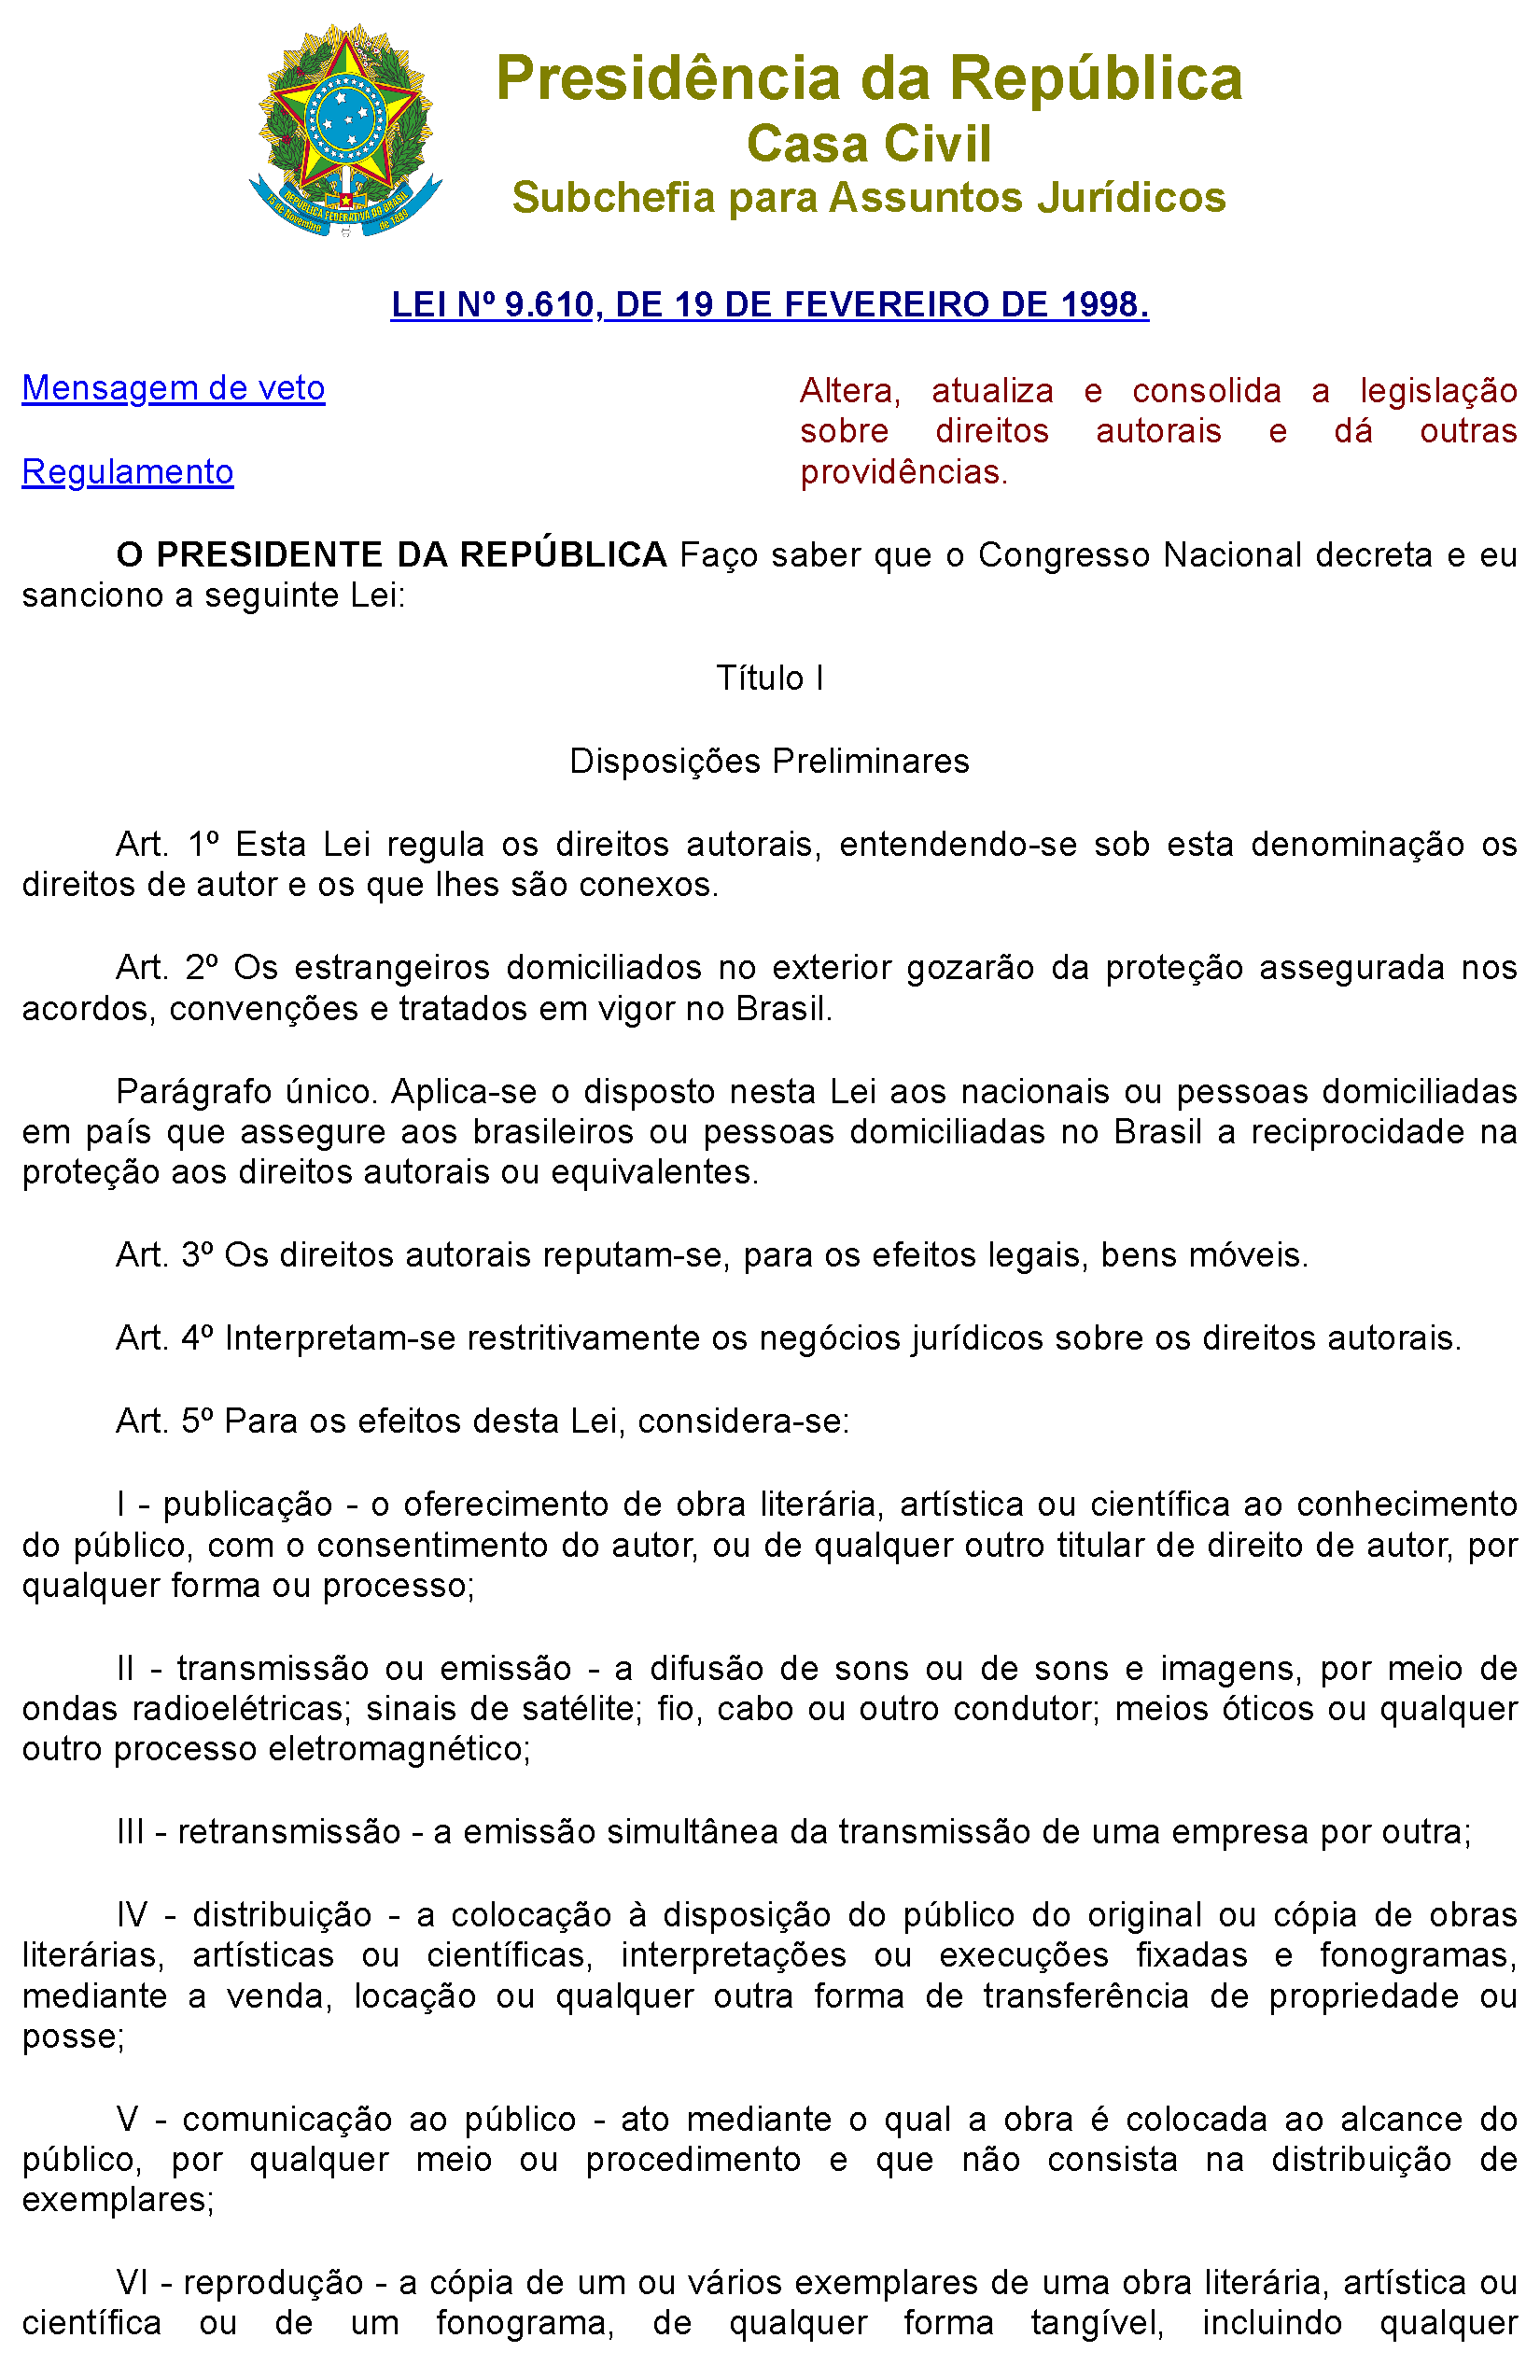
\includegraphics[%
  width  = 0.99999\textwidth,%
  height = 0.99999\textheight,%
  page   = 1,%
]{doc-law-n9610}

\newpage%

\noindent%
\includegraphics[%
  width  = 0.99999\textwidth,%
  height = 0.99999\textheight,%
  page   = 2,%
]{doc-law-n9610}

\sidebar{%
  Texto da lei na íntegra:\par%
  \href{https://www.planalto.gov.br/ccivil_03/leis/l9610.htm}{%
    
\includegraphics[height = 15mm]{doc-law-n9610-qr-code}%
  }%
}

%%%% ANEXO (B; ELEMENTO OPCIONAL)
%%
%% Texto ou documento não elaborado pelo autor, que serve de fundamentação,
%% comprovação e ilustração.

%% Locais (pastas) de ilustrações deste capítulo
\graphicspath{%
  {./Post-Textual/}%% Primário
  {./Post-Textual/Illustrations/}%% Secundário (descomentar se houver)
}

\chapter{Exemplos de Figura e Gráfico Produzidos em Aplicativos Específicos}%
\label{chpt:anx-b}

Figuras podem ser produzidas ou editadas com editores gráficos capazes de exportar a mesma em \ifbool{MakeAcr}{\intldescr{PS} (\intl{PS})}{\ENLang{PostScript} (PS)} ou, preferencialmente, \ifbool{MakeAcr}{\intl{EPS}}{EPS}.
O editor \href{https://www.xfig.org/}{Xfig\LinkIcon} é adequado para a maioria dos casos, mas outras opções para produção ou edição de diversas ilustrações são: \href{https://www.gimp.org/}{\ifbool{MakeAcr}{\intldescr{GIMP} (\intldescr+{GIMP} \textemdash\ \intl{GIMP})}{Programa de Manipulação de Imagem GNU (\ENLang*{GNU Image Manipulation Program} \textemdash\ GIMP)}\LinkIcon} e \href{http://dia-installer.de/}{Dia\LinkIcon}.
Este último é um editor orientado a diagramas (\ifbool{MakeAcr}{\intldescr{UML}\footnote{\IntlDescr+{UML} (\intl{UML})}}{Linguagem de Modelagem Unificada\footnote{\ENLang*{Unified Modeling Language} (UML)}}, fluxograma, etc.) com capacidade de exportar para diversos formatos, como na \Cref{fig:ex-uml} em \ifbool{MakeAcr}{\intl{PNG}}{PNG}~\cite{Larsson2020}.
Figuras em outros formatos (\ifbool{MakeAcr}{\intl{BMP}\footnote{\intldescr{BMP} (\intldescr+{BMP})}, \intl{GIF}\footnote{\intldescr{GIF} (\intldescr+{GIF})} e \intl{JPEG}}{BMP\footnote{Mapa de Bits (\ENLang*{Bitmap})}, GIF\footnote{Formato de Intercâmbio de Gráficos (\ENLang*{Graphics Interchange Format})} e JPEG}) podem ser convertidas para \ifbool{MakeAcr}{\intl{EPS}}{EPS} usando o aplicativo \href{https://github.com/jasper-software/xv.git}{XV\LinkIcon}, entre outros.
Este aplicativo não lista o \ifbool{MakeAcr}{\intl{EPS}}{EPS} dentre aqueles que consegue manipular, mas selecionando-se o \ifbool{MakeAcr}{\intl{PS}}{PS} e fornecendo-se a extensão \texttt{eps} ao nome do arquivo, o \ifbool{MakeAcr}{\intl{EPS}}{EPS} é produzido.

\begin{figure}[!htbp]
\SetCaptionWidth{\textwidth}
\caption[%
  Outro exemplo de figura (UML), produzida no editor gráfico Dia%
]{%
  Outro exemplo de figura (\ifbool{MakeAcr}{\intl{UML}}{UML}), produzida no editor gráfico \href{http://dia-installer.de/}{Dia\LinkIcon}%
}%
\label{fig:ex-uml}
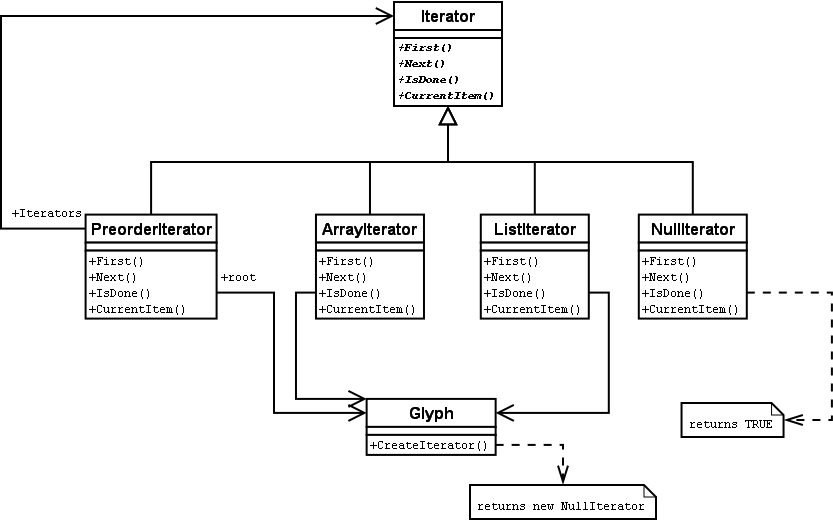
\includegraphics[width = \CaptionWidth]{fig-ex-uml}
\SourceOrNote{\textcite{Larsson2020}}
\end{figure}

Gráficos são produzidos com aplicativos capazes de exportar nos formatos \ifbool{MakeAcr}{\intl{PS} ou \intl{EPS}}{PS ou EPS}.
A ferramenta \href{http://www.gnuplot.info/}{gnuplot\LinkIcon} é uma das mais usadas para isto.
Uma vez no formato \ifbool{MakeAcr}{\intl{EPS}}{EPS}, gráficos são inseridos no texto, tal como figuras (ver \Cref{grph:ex-gnuplot}).

\begin{graph}[!htbp]
\SetCaptionWidth{0.7\textwidth}
\begin{minipage}{\CaptionWidth}
\caption[%
  Outro exemplo de gráfico, produzido em gnuplot a partir de arquivo de \ENLang*{script}%
]{%
  Outro exemplo de gráfico, produzido em gnuplot a partir de arquivo de \ENLang*{script}\footnote{\texttt{grph-ex-gnuplot.plt} em \texttt{./Post-Textual/Illustrations/}.}%
}%
\label{grph:ex-gnuplot}
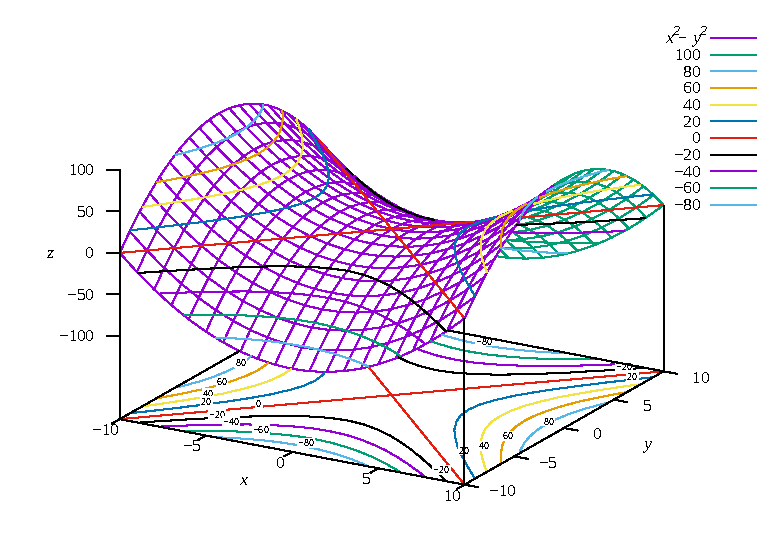
\includegraphics[width = \CaptionWidth]{grph-ex-gnuplot}
\end{minipage}
\SourceOrNote{adaptado de \textcite{Gnuplot2023}}
\end{graph}

\section{Título de seção secundária de anexo}%
\label{sect:anx-b2}

Exemplo de seção secundária de anexo (\Cref{sect:anx-b2}).

\subsection{Título de seção terciária de anexo}%
\label{ssect:anx-b3}

Exemplo de seção terciária de anexo (\Cref{ssect:anx-b3}).

\subsubsection{Título de seção quaternária de anexo}%
\label{sssect:anx-b4}

Exemplo de seção quaternária de anexo (\Cref{sssect:anx-b4}).

\paragraph{Título de seção quinária de anexo}%
\label{prgh:anx-b5}

Exemplo de seção quinária de anexo (\Cref{prgh:anx-b5}).

\subparagraph{Título de parágrafo (divisão de seção quinária) de anexo}%
\label{sprgh:anx-b6}

exemplo de parágrafo (divisão de seção quinária) de anexo (\Cref{sprgh:anx-b6}).

\end{Annexes}

%% Índice Remissivo (elemento opcional)
%%%% Opção 1 (makeindex, i.e., \index{...}, \Index{...}, etc.)
% \PrintIndex%
%%%% Opção 2 (manual; editar o {Arquivo} para alterar)
% %%%% ÍNDICE REMISSIVO (ELEMENTO OPCIONAL)
%%
%% Lista de palavras ou frases, ordenadas segundo determinado critério (e.g.,
%% alfabético), que localiza e remete para as informações contidas no texto.
\begin{RemissiveIndex}
\item \ensuremath{\vec{\nabla}} \see{operador gradiente}{999}
\item \ensuremath{\DottedCircle^0} \see{valor inicial}{999}
\item \ensuremath{\DottedCircle_\mathrm{S}} \see{fase sólida}{999}
\item \ensuremath{\theta} \see{inclinação}{999}
\item 1D \see{unidimensional}{999}
\indexspace%
\item alínea, \hyperpage{26}
\subitem subalínea, \hyperpage{26}
\item art.\ \see{artigo}{999}
\item artigo, \hyperpage{28}, \hyperpage{38}, \hyperpage{51}
\indexspace%
\item camundongo \see{rato}{999}
\item casa, \hyperpage{43}
\subitem janela, \hyperpage{43}
\subsubitem metal, \hyperpage{43}
\subitem porta, \hyperpage{43}
\subsubitem madeira, \hyperpage{43}
\item citação, \hyperpage{23, 24}, \hyperpage{27--29}, \hyperpage{41}
\subitem direta, \hyperpage{23, 24}, \hyperpage{28, 29}, \hyperpage{41}
\subitem indireta, \hyperpage{27}
\subsubitem explícita, \hyperpage{27}
\subsubitem implícita, \hyperpage{27}
\indexspace%
\item dissertação, \hyperpage{20}, \hyperpage{28}
\indexspace%
\item equilíbrio da configuração, \hyperpage{41}
\item espaçamento, \hyperpage{24}
\subitem de 1,5, \hyperpage{24}
\subitem entre linhas, \hyperpage{24}
\subitem entre parágrafos, \hyperpage{24}
\subitem simples, \hyperpage{24}
\indexspace%
\item fase sólida, \hyperpage{39}
\indexspace%
\item inclinação, \hyperpage{39}
\indexspace%
\item NBR \see{Norma Brasileira}{999}
\item Norma Brasileira, \hyperpage{22}
\item número de Reynolds, \hyperpage{39}
\indexspace%
\item operador gradiente, \hyperpage{39}
\indexspace%
\item pai, \hyperpage{41}, \hyperpage{51}
\subitem componente, \hyperpage{41}, \hyperpage{51}
\subitem filho, \hyperpage{41}, \hyperpage{51}
\indexspace%
\item ratazana \seealso{rato}{999}
\item rato, \hyperpage{43}
\subitem doméstico, \hyperpage{43}
\item \ensuremath{\mathrm{Re}} \see{número de Reynolds}{999}
\indexspace%
\item sistema operacional, \hyperpage{44}
\subitem Linux, \hyperpage{44}
\subitem macOS, \hyperpage{44}
\subitem Windows, \hyperpage{44}
\indexspace%
\item TCC \see{Trabalho de Conclusão de Curso}{999}
\item tese, \hyperpage{20}, \hyperpage{28}
\item \TeX, \hyperpage{21}, \hyperpage{41}, \hyperpage{45}, \hyperpage{51}, \hyperpage{54}
\subitem \LaTeX, \hyperpage{20, 21}, \hyperpage{23}, \hyperpage{29--31}, \hyperpage{37}, \hyperpage{40, 41}, \hyperpage{44--46}, \hyperpage{51}, \hyperpage{54}
\subsubitem biber, \hyperpage{40}
\subsubitem Bib\LaTeX, \hyperpage{27}, \hyperpage{40}, \hyperpage{51}
\subsubitem Bib\LaTeX-abnt, \hyperpage{27}, \hyperpage{40}
\subsubitem Bib\TeX, \hyperpage{40}, \hyperpage{51}
\subsubitem memoir, \hyperpage{20}, \hyperpage{25}, \hyperpage{32}, \hyperpage{45}
\subsubitem Overleaf, \hyperpage{44}
\subsubitem Papeeria, \hyperpage{44}
\subsubitem TeXlipse, \hyperpage{44}
\subsubitem Texmaker, \hyperpage{20}, \hyperpage{44}
\subsubitem {\TeX}Page, \hyperpage{44}
\subsubitem \UTFPR-Thesis, \hyperpage{20}, \hyperpage{25}, \hyperpage{27}, \hyperpage{41}
\item Trabalho de Conclusão de Curso, \hyperpage{20}
\indexspace%
\item unidimensional, \hyperpage{38}
\indexspace%
\item \ensuremath{V} \see{velocidade}{999}
\item valor inicial, \hyperpage{39}
\item velocidade, \hyperpage{39}
\end{RemissiveIndex}


%% Fim do documento
\end{document}

%% Nota: o arquivo final (PDF) pode ser convertido para PDF/A usando diversas
%% ferramentas, por exemplo:
%%   https://www.pdfforge.org/online/en/pdf-to-pdfa
